\documentclass[12pt,a4paper,oneside]{report}
\usepackage[a4paper,left=3cm,right=2.5cm,top=2.5cm,bottom=2.5cm]{geometry}
\usepackage{fontspec}
\setmainfont{Times New Roman}
\usepackage{polyglossia}
\setdefaultlanguage{vietnamese}
\setotherlanguage{english}
\usepackage{setspace}
\onehalfspacing
\usepackage{graphicx,booktabs,tabularx,longtable,array,multirow}
\usepackage{amsmath,amssymb}
\usepackage{float,caption,subcaption}
\usepackage{fancyhdr}
\usepackage{enumitem}
\usepackage{listings,xcolor}
\usepackage{hyperref}
\usepackage{xurl}
\usepackage{microtype}
\usepackage{titlesec}
\usepackage{tocloft}
\hypersetup{hidelinks,pdftitle={Bao cao van hanh he thong hoc may - Bao tri du doan},pdfauthor={Luong Trung Kien, Ha Vinh Phuoc, Nguyen Van Tuan Tu}}
\graphicspath{{figures/}{../reports/figures/}}
\captionsetup{font=small,labelfont=bf}
\setlist{itemsep=2pt,topsep=3pt}
\setlength{\parindent}{1.2cm}
\setlength{\parskip}{2pt}
\setlength{\headheight}{14pt}
\emergencystretch=3em
\renewcommand{\contentsname}{Mục lục}
\renewcommand{\listfigurename}{Danh mục hình}
\renewcommand{\listtablename}{Danh mục bảng}
\renewcommand{\bibname}{Tài liệu tham khảo}
\renewcommand{\figurename}{Hình}
\renewcommand{\tablename}{Bảng}
\pagestyle{fancy}
\fancyhf{}
\fancyhead[L]{\small Báo cáo môn Vận hành hệ thống học máy}
\fancyhead[R]{\small Bảo trì dự đoán}
\fancyfoot[C]{\thepage}
\renewcommand{\headrulewidth}{0.4pt}
\lstdefinestyle{code}{basicstyle=\ttfamily\footnotesize,breaklines=true,frame=single,framesep=5pt,showstringspaces=false,backgroundcolor=\color{gray!5},keywordstyle=\color{blue!60!black}}
\lstset{style=code}
\newcommand{\src}[1]{\nolinkurl{#1}}
\newcommand{\dataset}{AI4I 2020}
\newcommand{\project}{Hệ thống MLOps cho bảo trì dự đoán}

\begin{document}
\pagenumbering{roman}
\begin{titlepage}
\centering
{\large BỘ GIÁO DỤC VÀ ĐÀO TẠO\par}
\vspace{0.4cm}
{\large BÁO CÁO HỌC PHẦN\par}
\vspace{2.8cm}
{\Large\bfseries VẬN HÀNH HỆ THỐNG HỌC MÁY\par}
\vspace{1.0cm}
{\Huge\bfseries HỆ THỐNG MLOps CHO BẢO TRÌ DỰ ĐOÁN\par}
\vspace{0.4cm}
{\Large Phân loại trạng thái hỏng máy trên dữ liệu AI4I 2020\par}
\vspace{2cm}
\begin{tabular}{ll}
\textbf{Nhóm thực hiện:} & Lương Trung Kiên --- 20250386E\\
& Hà Vĩnh Phước --- 20241617E\\
& Nguyễn Văn Tuấn Tú --- 20260079E\\
\textbf{Mã nguồn:} & \url{https://github.com/kienluongzero-hue/MLops}
\end{tabular}
\vfill
{\large Tháng 11 năm 2026\par}
\end{titlepage}
\clearpage
\chapter*{Tóm tắt}
\addcontentsline{toc}{chapter}{Tóm tắt}
Báo cáo trình bày quá trình xây dựng một hệ thống học máy có thể tái tạo, kiểm thử và quan sát được cho bài toán phân loại trạng thái hỏng máy. Nguồn dữ liệu là bộ \dataset{} của UCI gồm 10.000 bản ghi mô phỏng và 339 bản ghi hỏng máy. Nhóm xây dựng đường xử lý từ tải dữ liệu, chia tập có phân tầng, tiền xử lý, so sánh ba mô hình, theo dõi thí nghiệm đến đóng gói dịch vụ dự đoán và giám sát sự thay đổi phân phối đầu vào.

Ba mô hình được so sánh gồm Logistic Regression, Random Forest và XGBoost. XGBoost đạt average precision 0,780 trên tập validation và được chọn trước khi đánh giá tập test. Ngưỡng xác suất 0,15 được chọn trên validation bằng điểm $F_2$. Trên 2.000 bản ghi test, mô hình đạt average precision 0,825, recall 0,794, precision 0,614; trong 68 trường hợp hỏng, hệ thống phát hiện đúng 54 và bỏ sót 14. Các kết quả này chỉ áp dụng cho cách chia tập và bộ dữ liệu mô phỏng đang xét.

Pipeline DVC quản lý các bước tải dữ liệu và huấn luyện; MLflow lưu tham số cùng chỉ số; FastAPI phục vụ suy luận trong Docker; GitHub Actions chạy kiểm thử; công cụ giám sát so sánh một lô dữ liệu mới với tập train. Thử nghiệm dịch chuyển chủ động trên ba thuộc tính làm hệ thống phát cảnh báo. Báo cáo phân tích các quyết định kỹ thuật, phép đo, khả năng tái tạo, rủi ro rò rỉ nhãn và giới hạn khi chuyển sang dữ liệu máy thật.

\noindent\textbf{Từ khóa:} MLOps, bảo trì dự đoán, AI4I, DVC, MLflow, XGBoost, giám sát dữ liệu.
\clearpage
\chapter*{Lời cam đoan và phạm vi}
\addcontentsline{toc}{chapter}{Lời cam đoan và phạm vi}
Các số liệu thực nghiệm trong báo cáo được lấy từ mã nguồn, tệp dữ liệu và hiện vật chạy được lưu cùng repository, không phải số liệu từ môi trường sản xuất. Những phân tích về tác động vận hành là nhận định trong phạm vi bài tập; nhóm chưa kiểm chứng hiệu năng trên dây chuyền công nghiệp. Dữ liệu \dataset{} là dữ liệu tổng hợp, còn nhãn \src{Machine failure} mô tả hỏng tại bản ghi hiện tại. Vì thế thuật ngữ ``bảo trì dự đoán'' trong tên đề tài chỉ bối cảnh ứng dụng, không hàm ý dự báo tuổi thọ còn lại hoặc cảnh báo trước một khoảng thời gian xác định.

Bản báo cáo có thể được biên dịch lại từ mã LaTeX. Những hình và bảng số liệu phụ thuộc thực nghiệm được tạo bằng \src{latex-report/generate_assets.py}; nguồn số liệu là \src{data/raw/ai4i2020.csv}, \src{artifacts/metrics.json} và các báo cáo giám sát. Mỗi khi thay đổi pipeline, cần chạy lại chương trình tạo bằng chứng trước khi biên dịch.
\clearpage
\tableofcontents
\clearpage
\listoffigures
\clearpage
\listoftables
\clearpage
\pagenumbering{arabic}
\chapter{Giới thiệu đề tài}
\section{Bối cảnh}
Thiết bị trong một hệ thống sản xuất tạo ra các phép đo về nhiệt độ, tốc độ quay, mô-men xoắn và mức hao mòn. Nếu có thể nhận ra các trạng thái liên quan đến hỏng máy từ những phép đo này, người vận hành có thêm tín hiệu để kiểm tra thiết bị. Tuy nhiên, một mô hình có chỉ số tốt trong notebook chưa đủ để sử dụng có hệ thống. Cần biết dữ liệu nào đã được dùng, phiên bản mã nào sinh ra mô hình, ngưỡng ra quyết định ra sao, dịch vụ có nhận đúng cấu trúc dữ liệu hay không và phân phối dữ liệu mới có khác dữ liệu huấn luyện không. Đây là lý do đề tài đặt trọng tâm vào vòng đời mô hình bên cạnh thuật toán phân loại. Những vấn đề về phụ thuộc dữ liệu và cấu hình trong hệ thống ML cũng được Sculley và cộng sự mô tả như một dạng nợ kỹ thuật \cite{sculley2015}.

Nhóm chọn \dataset{} do UCI công bố \cite{uci2020}. Dữ liệu có 10.000 quan sát và một nhãn nhị phân về hỏng máy; sáu thuộc tính đầu vào có ý nghĩa trực quan. Quy mô vừa đủ để huấn luyện và chạy lại pipeline trên máy cá nhân. Dữ liệu là mô phỏng, điều này giúp khảo sát quy trình kỹ thuật nhưng giới hạn khả năng suy rộng kết quả sang thiết bị thật. Tên gọi predictive maintenance trong nguồn dữ liệu và tên dự án được giữ để phản ánh bối cảnh, còn bài toán được đo chính xác trong báo cáo là \emph{phân loại trạng thái hỏng của từng bản ghi}.

\section{Bài toán và câu hỏi nghiên cứu}
Gọi $x_i$ là sáu phép đo và thuộc tính loại sản phẩm của bản ghi thứ $i$, $y_i\in\{0,1\}$ là nhãn \src{Machine failure}. Mục tiêu mô hình là ước lượng $p_i=P(y_i=1\mid x_i)$ và phát cảnh báo nếu $p_i\geq t$. Vì chỉ 3,39\% bản ghi mang nhãn hỏng, chọn ngưỡng $t$ và cách đo kết quả quan trọng không kém lựa chọn thuật toán.

Báo cáo trả lời bốn câu hỏi. Thứ nhất, dữ liệu và nhãn có những đặc điểm nào khiến bài toán khó? Thứ hai, trong ba họ mô hình được thử, mô hình nào phù hợp nhất theo average precision trên tập validation? Thứ ba, một người khác có thể chạy lại chuỗi tải dữ liệu, huấn luyện và phục vụ kết quả bằng các thành phần nào? Thứ tư, hệ thống phản ứng thế nào khi phân phối đầu vào của một lô mới thay đổi có chủ đích? Các câu hỏi được trả lời bằng hiện vật chạy thực tế, thay vì mô tả kiến trúc dự kiến.

\section{Mục tiêu và sản phẩm}
Mục tiêu thứ nhất là tạo một quy trình huấn luyện có thể tái tạo: dữ liệu nguồn xác định được, phép chia tập cố định, tiền xử lý nằm trong pipeline của mô hình và quyết định lựa chọn dựa trên validation. Mục tiêu thứ hai là tạo dịch vụ dự đoán với hợp đồng đầu vào rõ ràng và môi trường đóng gói bằng Docker. Mục tiêu thứ ba là lưu dấu vết thực nghiệm và kiểm tra tự động. Mục tiêu cuối là theo dõi độ lệch phân phối đầu vào trên các lô dữ liệu, đồng thời phân biệt cảnh báo chất lượng dữ liệu với đánh giá chất lượng dự đoán.

Sản phẩm cụ thể của repository là mã Python, \src{dvc.yaml} và \src{dvc.lock}, tệp cấu hình phụ thuộc, kiểm thử, Dockerfile, các hiện vật được sinh bởi pipeline, báo cáo thực nghiệm và tài liệu này. Mô hình nhị phân \src{model.joblib} được sinh cục bộ khi huấn luyện; Git chỉ lưu mã và định nghĩa pipeline. Cách tổ chức này giúp người đọc thấy rõ bước nào là đầu vào, bước nào là sản phẩm có thể tái tạo.

\section{Phạm vi và giả định}
Hệ thống xử lý một bộ dữ liệu bảng tĩnh và một yêu cầu API cho mỗi bản ghi. Các lô giám sát là tệp CSV, chưa phải luồng dữ liệu thời gian thực. Báo cáo không gán chi phí tiền tệ cho một cảnh báo sai hoặc một lỗi bỏ sót vì chưa có thông tin kinh doanh để xác định chi phí. Việc ưu tiên recall thông qua $F_2$ là một lựa chọn minh họa: trong ngữ cảnh bảo trì, bỏ sót một trạng thái hỏng có thể đáng quan tâm, nhưng quyết định thực tế phải do đơn vị vận hành xác lập.

Dữ liệu không chứa dấu thời gian, mã thiết bị có thể theo dõi lâu dài hoặc thời điểm hỏng trong tương lai. Vì thế phép chia ngẫu nhiên có phân tầng ở đây chỉ kiểm tra khả năng phân loại trên các bản ghi cùng phân phối giả định. Nó không chứng minh mô hình dự báo sớm cho thiết bị chưa từng thấy. Phần thảo luận sẽ quay lại giới hạn này khi diễn giải kết quả và đề xuất bước tiếp theo.

\section{Bố cục báo cáo}
Chương 2 trình bày cơ sở về bài toán mất cân bằng, chỉ số đánh giá và các công cụ MLOps. Chương 3 phân tích bộ dữ liệu và rủi ro rò rỉ nhãn. Chương 4 mô tả thiết kế hệ thống; chương 5 trình bày huấn luyện và quy tắc chọn mô hình. Chương 6 đi vào hiện thực DVC, MLflow, API, Docker và CI. Chương 7 ghi nhận kết quả mô hình cùng thử nghiệm giám sát. Chương 8 kết luận, nêu giới hạn và hướng phát triển. Các phụ lục đưa ra lệnh chạy lại và hợp đồng API.


\chapter{Cơ sở lý thuyết và công nghệ}
\section{Phân loại nhị phân trong dữ liệu mất cân bằng}
Với bài toán nhị phân, một dự đoán có bốn khả năng: đúng âm (TN), dương giả (FP), âm giả (FN) và đúng dương (TP). Khi tỷ lệ dương thấp, accuracy có thể cao ngay cả khi mô hình luôn dự đoán không hỏng. Trên bộ dữ liệu này, mô hình luôn trả về không hỏng sẽ có accuracy 96,61\% nhưng recall bằng 0. Vì vậy nhóm tập trung vào khả năng xếp hạng các bản ghi hỏng và sự đánh đổi giữa cảnh báo sai với bỏ sót.

Precision và recall được tính theo
\begin{equation}
\mathrm{Precision}=\frac{TP}{TP+FP},\qquad
\mathrm{Recall}=\frac{TP}{TP+FN}.
\end{equation}
Điểm $F_\beta$ là trung bình điều hòa có trọng số:
\begin{equation}
F_\beta=(1+\beta^2)\frac{\mathrm{Precision}\cdot\mathrm{Recall}}{\beta^2\mathrm{Precision}+\mathrm{Recall}}.
\end{equation}
Với $\beta=2$, recall nhận trọng số lớn hơn precision. Chỉ số này phụ thuộc ngưỡng $t$; do đó chọn ngưỡng trên tập test sẽ làm sai lệch kết quả báo cáo. Trong quy trình của nhóm, $t$ chỉ được tối ưu trên validation.

Đường precision--recall mô tả hiệu năng khi thay đổi ngưỡng. \emph{Average precision} (AP) tổng hợp đường này theo mức tăng recall, không cần chốt trước một ngưỡng. Khi dữ liệu mất cân bằng, đường PR cho biết rõ hơn tỷ lệ dự báo hỏng thật trong số các cảnh báo; nghiên cứu của Saito và Rehmsmeier cũng chỉ ra lợi ích của đường PR trong bối cảnh này \cite{saito2015}. Báo cáo dùng tên ``PR-AUC'' trong bảng để dễ đọc, song số liệu cụ thể được tính bằng \src{sklearn.metrics.average_precision_score}; AP và diện tích nội suy hình thang không hoàn toàn đồng nhất. ROC-AUC vẫn được báo cáo để bổ sung góc nhìn về thứ hạng dương--âm, chứ không thay thế precision và recall tại ngưỡng vận hành.

\section{Ba họ mô hình được khảo sát}
Logistic Regression ước lượng xác suất thông qua hàm sigmoid của tổ hợp tuyến tính đặc trưng. Đây là đường chuẩn dễ diễn giải và huấn luyện nhanh. Tùy chọn \src{class_weight="balanced"} tăng trọng số tương đối cho lớp hỏng trong quá trình khớp mô hình. Dù vậy, quan hệ giữa cảm biến và hỏng máy có thể phi tuyến, khiến mô hình tuyến tính khó nắm bắt đủ.

Random Forest là tập hợp nhiều cây quyết định được huấn luyện trên các mẫu bootstrap và lựa chọn tập con thuộc tính, rồi tổng hợp dự đoán \cite{breiman2001}. Mô hình có thể học tương tác phi tuyến và ít cần giả định dạng hàm. Trong triển khai này có 200 cây, mỗi lá tối thiểu hai quan sát và trọng số lớp được cân bằng theo từng mẫu bootstrap. Các lựa chọn này được cố định trước khi nhìn tập test; chúng không phải kết quả của tìm kiếm siêu tham số toàn diện.

XGBoost xây dựng tuần tự các cây tăng cường gradient, tối ưu hàm mất mát có điều chuẩn và hỗ trợ nhiều tối ưu hóa tính toán \cite{chen2016}. Nhóm sử dụng 250 cây, độ sâu tối đa 4, tốc độ học 0,05, tỷ lệ lấy mẫu bản ghi và thuộc tính cùng bằng 0,9. Trong bộ ba ứng viên, XGBoost là mô hình phức tạp hơn, do đó cần đối chiếu trên validation và đánh giá riêng trên test. Giá trị độ quan trọng thuộc tính của mô hình không phải bằng chứng về quan hệ nhân quả.

\section{Tách dữ liệu và kiểm soát rò rỉ}
Ba tập có nhiệm vụ khác nhau. Train dùng để khớp bộ biến đổi và tham số mô hình. Validation dùng để so sánh ứng viên và chọn ngưỡng. Test được giữ lại cho một lần đánh giá kết quả đã chọn. Hàm \src{train_test_split} với \src{stratify} giữ tỷ lệ lớp gần nhau giữa các tập; \src{random_state=42} làm phép chia lặp lại được. Pipeline của scikit-learn gói OneHotEncoder, StandardScaler và bộ phân loại để các tham số biến đổi chỉ được học trên train.

Rò rỉ nhãn có thể xuất hiện ngay trong schema. Năm cột TWF, HDF, PWF, OSF, RNF mô tả các chế độ lỗi liên quan trực tiếp đến nhãn mục tiêu; đưa chúng vào đầu vào sẽ cho mô hình thông tin mà dịch vụ suy luận bình thường không có. Hai cột định danh \src{UDI} và \src{Product ID} cũng bị loại bỏ để tránh học trật tự hoặc mã sản phẩm thay vì tín hiệu cảm biến. Một danh sách cho phép sáu thuộc tính được dùng chung bởi huấn luyện, API và giám sát giúp tránh bất đồng schema.

\section{MLOps và các thành phần được chọn}
MLOps ở đây được hiểu là thực hành quản lý toàn bộ đường đi từ dữ liệu đến suy luận và quan sát. DVC định nghĩa các giai đoạn có phụ thuộc và đầu ra; khi chạy \src{dvc repro}, công cụ kiểm tra thay đổi và chạy lại bước cần thiết \cite{dvc}. DVC không tự bảo đảm khả năng tải lại dữ liệu nếu nguồn bên ngoài biến mất. Vì thế báo cáo ghi SHA-256 của CSV gốc, còn repository chưa cấu hình DVC remote để phân phối cache dữ liệu và mô hình.

MLflow Tracking lưu tham số, chỉ số và hiện vật của từng lượt chạy trong một kho theo dõi \cite{mlflow}. Với cấu hình hiện tại, kho là SQLite cục bộ. Điều này đủ để so sánh thí nghiệm trên một máy nhưng chưa tạo một máy chủ thí nghiệm chung cho nhóm. FastAPI dùng khai báo dữ liệu để xác thực JSON đầu vào và cung cấp mô tả OpenAPI \cite{fastapi}. Docker đóng gói môi trường chạy API thành image từ Dockerfile \cite{docker}. GitHub Actions thực thi kiểm thử khi push hoặc mở pull request \cite{actions}. Vai trò các công cụ là bổ trợ nhau; không công cụ nào tự thay thế việc đo chất lượng mô hình hay kiểm tra dữ liệu đầu vào.

\section{Giám sát sự thay đổi phân phối}
Một mô hình được huấn luyện trên phân phối tham chiếu $P_{\mathrm{train}}(X)$; các lô mới có thể đến từ $P_{\mathrm{new}}(X)$ khác. Công cụ giám sát của nhóm so sánh từng thuộc tính, không ước lượng trực tiếp độ chính xác mô hình. Với biến phân loại \src{Type}, khoảng cách total variation là
\begin{equation}
D_{\mathrm{TV}}(P,Q)=\frac{1}{2}\sum_{c\in\{L,M,H\}}|P(c)-Q(c)|.
\end{equation}
Với các thuộc tính số, thống kê Kolmogorov--Smirnov hai mẫu là
\begin{equation}
D_{n,m}=\sup_x\left|\widehat F_n(x)-\widehat G_m(x)\right|,
\end{equation}
trong đó $\widehat F_n$ và $\widehat G_m$ là các hàm phân phối tích lũy thực nghiệm. Triển khai dùng \src{scipy.stats.ks_2samp} \cite{scipyks}. Ngưỡng cảnh báo được chọn để minh họa: TV $\geq0,10$; KS $\geq0,20$ đồng thời $p<0,01$. Đây không phải ngưỡng đã hiệu chuẩn bằng dữ liệu vận hành thật. Khi kiểm tra nhiều thuộc tính, nguy cơ cảnh báo ngẫu nhiên cũng cần được xem xét nếu triển khai quy mô lớn.


\chapter{Bộ dữ liệu và khảo sát dữ liệu}
\section{Nguồn gốc và khả năng sử dụng}
Bộ \dataset{} do Stephan Matzka công bố trên UCI Machine Learning Repository với DOI \url{10.24432/C5HS5C}, giấy phép CC BY 4.0 \cite{uci2020,matzka2020}. Tác giả xây dựng dữ liệu tổng hợp nhằm phản ánh một số tình huống bảo trì dự đoán. Đây là thuận lợi cho bài tập có thể chia sẻ công khai, đồng thời phải được nêu rõ khi diễn giải kết quả. Tệp CSV mà pipeline sử dụng có SHA-256 \src{dc6630cd9b1f0f853922fad78a1b6436570d3f1ec863f1dd5c4340ac56bc8a8e}. Hàm tải của dự án xác thực nguồn trước khi sử dụng, giúp phát hiện nếu nội dung tệp thay đổi ngoài dự kiến.

\section{Cấu trúc trường dữ liệu}
Tệp thực tế có 14 cột. \src{UDI} là số định danh dòng và \src{Product ID} là mã sản phẩm. \src{Type} nhận một trong ba giá trị L, M, H. Năm phép đo gồm nhiệt độ không khí, nhiệt độ quá trình, tốc độ quay, mô-men xoắn và thời gian hao mòn dụng cụ. \src{Machine failure} là nhãn tổng thể. Năm cột TWF, HDF, PWF, OSF và RNF mô tả chế độ hỏng. Tên \src{UDI} được ghi theo chính tệp CSV tải về; trang giới thiệu bộ dữ liệu dùng cách đặt tên có thể khác. Báo cáo ưu tiên schema của hiện vật thực nghiệm.

\begin{table}[H]\centering\caption{Các trường được đưa vào mô hình}\label{tab:features}
\begin{tabularx}{\textwidth}{p{4.8cm}p{2.5cm}X}\toprule
Trường & Kiểu & Ý nghĩa và xử lý\\\midrule
Type & Phân loại & Mã loại sản phẩm L/M/H; one-hot encoding\\
Air temperature [K] & Số thực & Nhiệt độ không khí; chuẩn hóa trên train\\
Process temperature [K] & Số thực & Nhiệt độ quá trình; chuẩn hóa trên train\\
Rotational speed [rpm] & Số nguyên & Tốc độ quay; chuẩn hóa trên train\\
Torque [Nm] & Số thực & Mô-men xoắn; chuẩn hóa trên train\\
Tool wear [min] & Số nguyên & Thời gian hao mòn; chuẩn hóa trên train\\\bottomrule
\end{tabularx}
\end{table}
Việc loại trừ các cột nguyên nhân hỏng là quyết định thiết kế quan trọng hơn việc thử thêm thuật toán. Chúng là các chỉ báo lỗi đã xác định, không phải thông số cảm biến độc lập trước quyết định. Nếu dùng chúng để dự báo \src{Machine failure}, bài toán huấn luyện sẽ khác hợp đồng API có sáu trường. Danh sách cho phép trong \src{features.py} khiến mã dừng ngay khi thiếu trường bắt buộc, nhãn không nhị phân hoặc loại sản phẩm không hợp lệ.

\section{Quy mô, cân bằng lớp và giá trị thiếu}
Tập có 10.000 dòng, không có giá trị thiếu trong 14 cột. Có 9.661 bản ghi không hỏng và 339 bản ghi hỏng, tương ứng tỷ lệ dương 3,39\%. Hình~\ref{fig:class} cho thấy chênh lệch đáng kể giữa hai lớp. Một số đo chỉ dựa trên số dự đoán đúng sẽ bị lớp đông chi phối, vì vậy báo cáo ưu tiên AP và các chỉ số từ ma trận nhầm lẫn.

\begin{figure}[H]\centering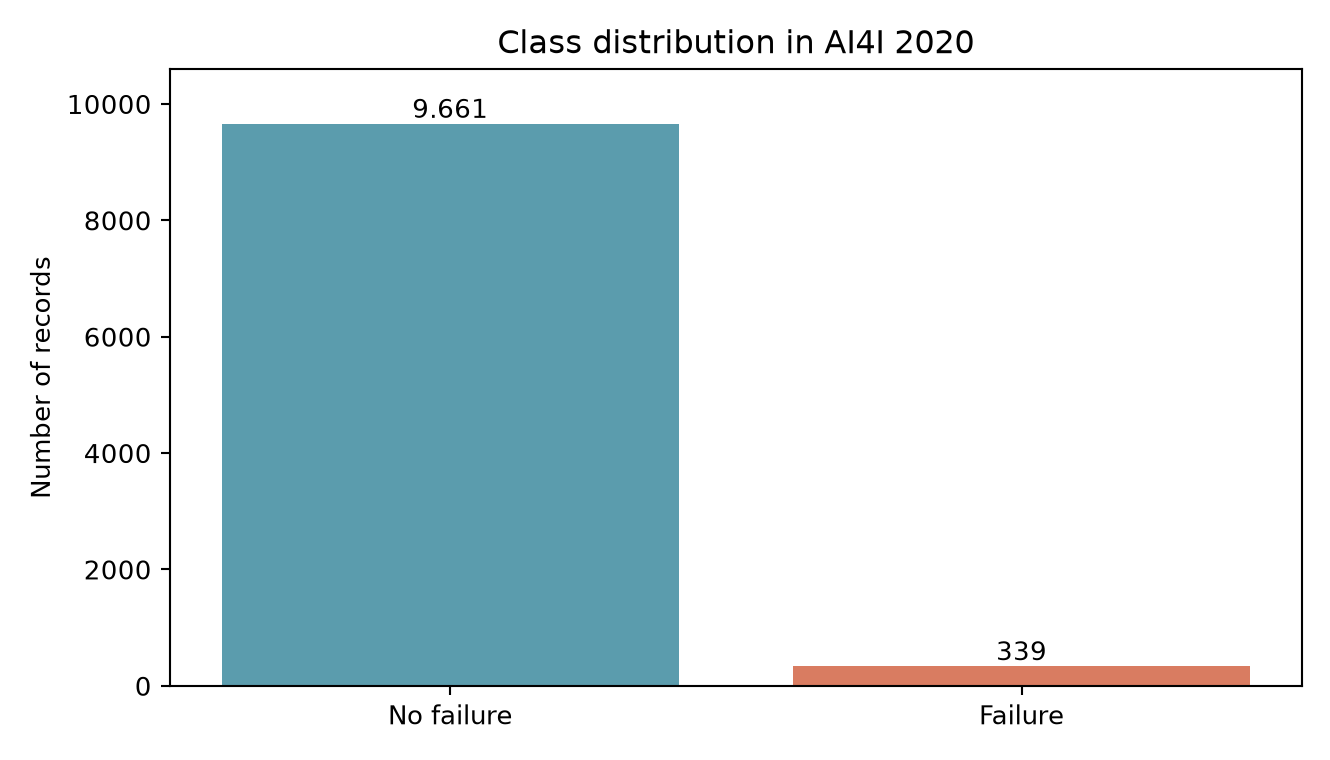
\includegraphics[width=.78\textwidth]{class_balance.png}\caption{Phân bố nhãn trong dữ liệu gốc. Nguồn: tính từ CSV đã xác thực SHA-256.}\label{fig:class}\end{figure}

\begin{table}[H]\centering\caption{Số lượng và tỷ lệ hỏng theo loại sản phẩm}\label{tab:type}
\begin{tabular}{lrrr}\toprule Loại & Số bản ghi & Số hỏng & Tỷ lệ hỏng\\\midrule
L & 6.000 & 235 & 3,92\% \\
M & 2.997 & 83 & 2,77\% \\
H & 1.003 & 21 & 2,09\% \\
\bottomrule

\end{tabular}\end{table}
Ba loại sản phẩm không có cùng số quan sát: L có 6.000, M có 2.997 và H có 1.003. Tỷ lệ lỗi theo nhóm trong Bảng~\ref{tab:type} là mô tả của dữ liệu, không chứng minh rằng một loại sản phẩm gây hỏng. Muốn kết luận nhân quả cần hiểu cơ chế sinh dữ liệu và kiểm soát các biến khác. Trong phục vụ mô hình, giá trị \src{Type} ngoài L/M/H bị API từ chối; bộ mã hóa vẫn cấu hình \src{handle_unknown="ignore"} để pipeline có hành vi xác định nếu được dùng trong ngữ cảnh khác.

\begin{figure}[H]\centering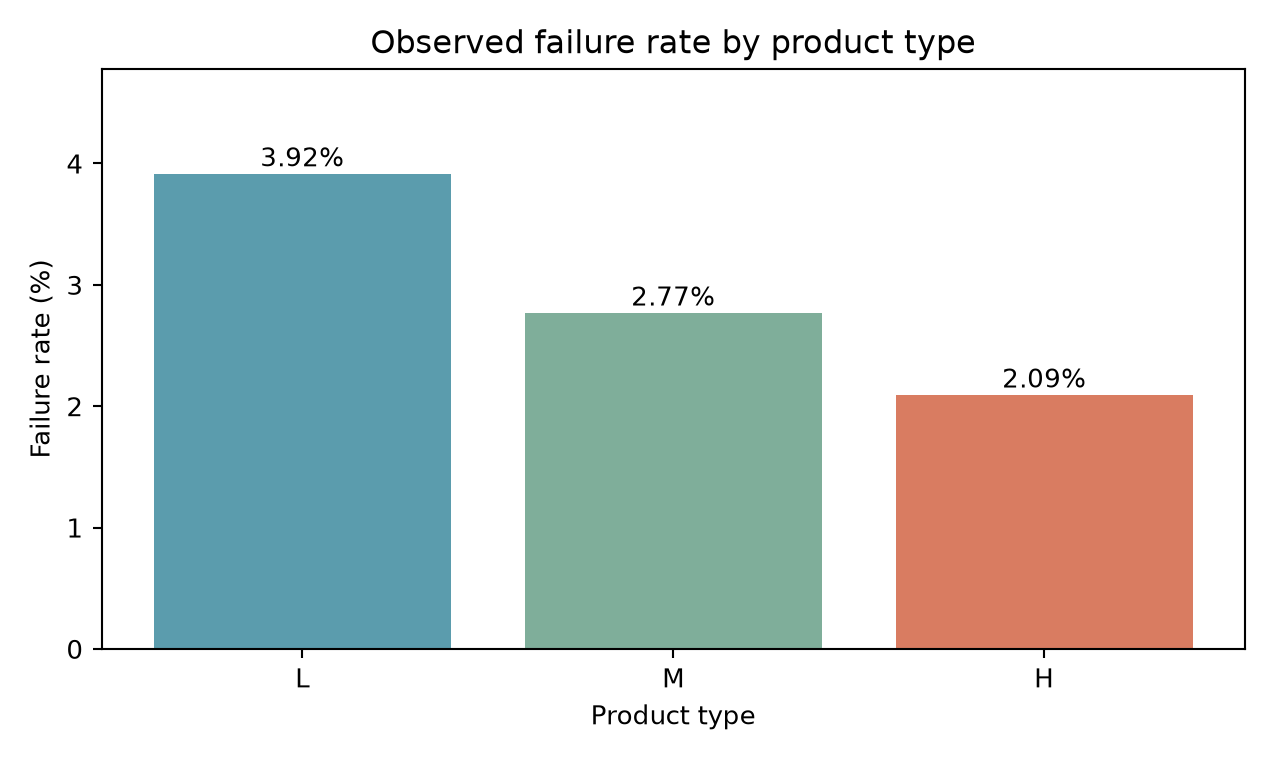
\includegraphics[width=.98\textwidth]{type_failure_rate.png}\caption{Quy mô và tỷ lệ bản ghi hỏng theo loại sản phẩm.}\label{fig:type}\end{figure}

\section{Phân phối cảm biến và chế độ hỏng}
Hình~\ref{fig:sensors} đặt cạnh phân phối của năm biến số theo nhãn. Các biểu đồ giúp nhìn vùng giá trị chồng lấn và những khác biệt dễ thấy; chúng không thể hiện quan hệ có điều kiện giữa các biến. Từ tệp dữ liệu, trung bình mô-men xoắn của nhóm hỏng là 50,17 Nm so với 39,63 Nm của nhóm không hỏng; hao mòn trung bình lần lượt là 143,78 và 106,69 phút. Nhiệt độ không khí trung bình là 300,89 K ở nhóm hỏng và 299,97 K ở nhóm bình thường. Những con số này mô tả tương quan biên và không xác định một quy tắc chẩn đoán đơn lẻ.

\begin{figure}[H]\centering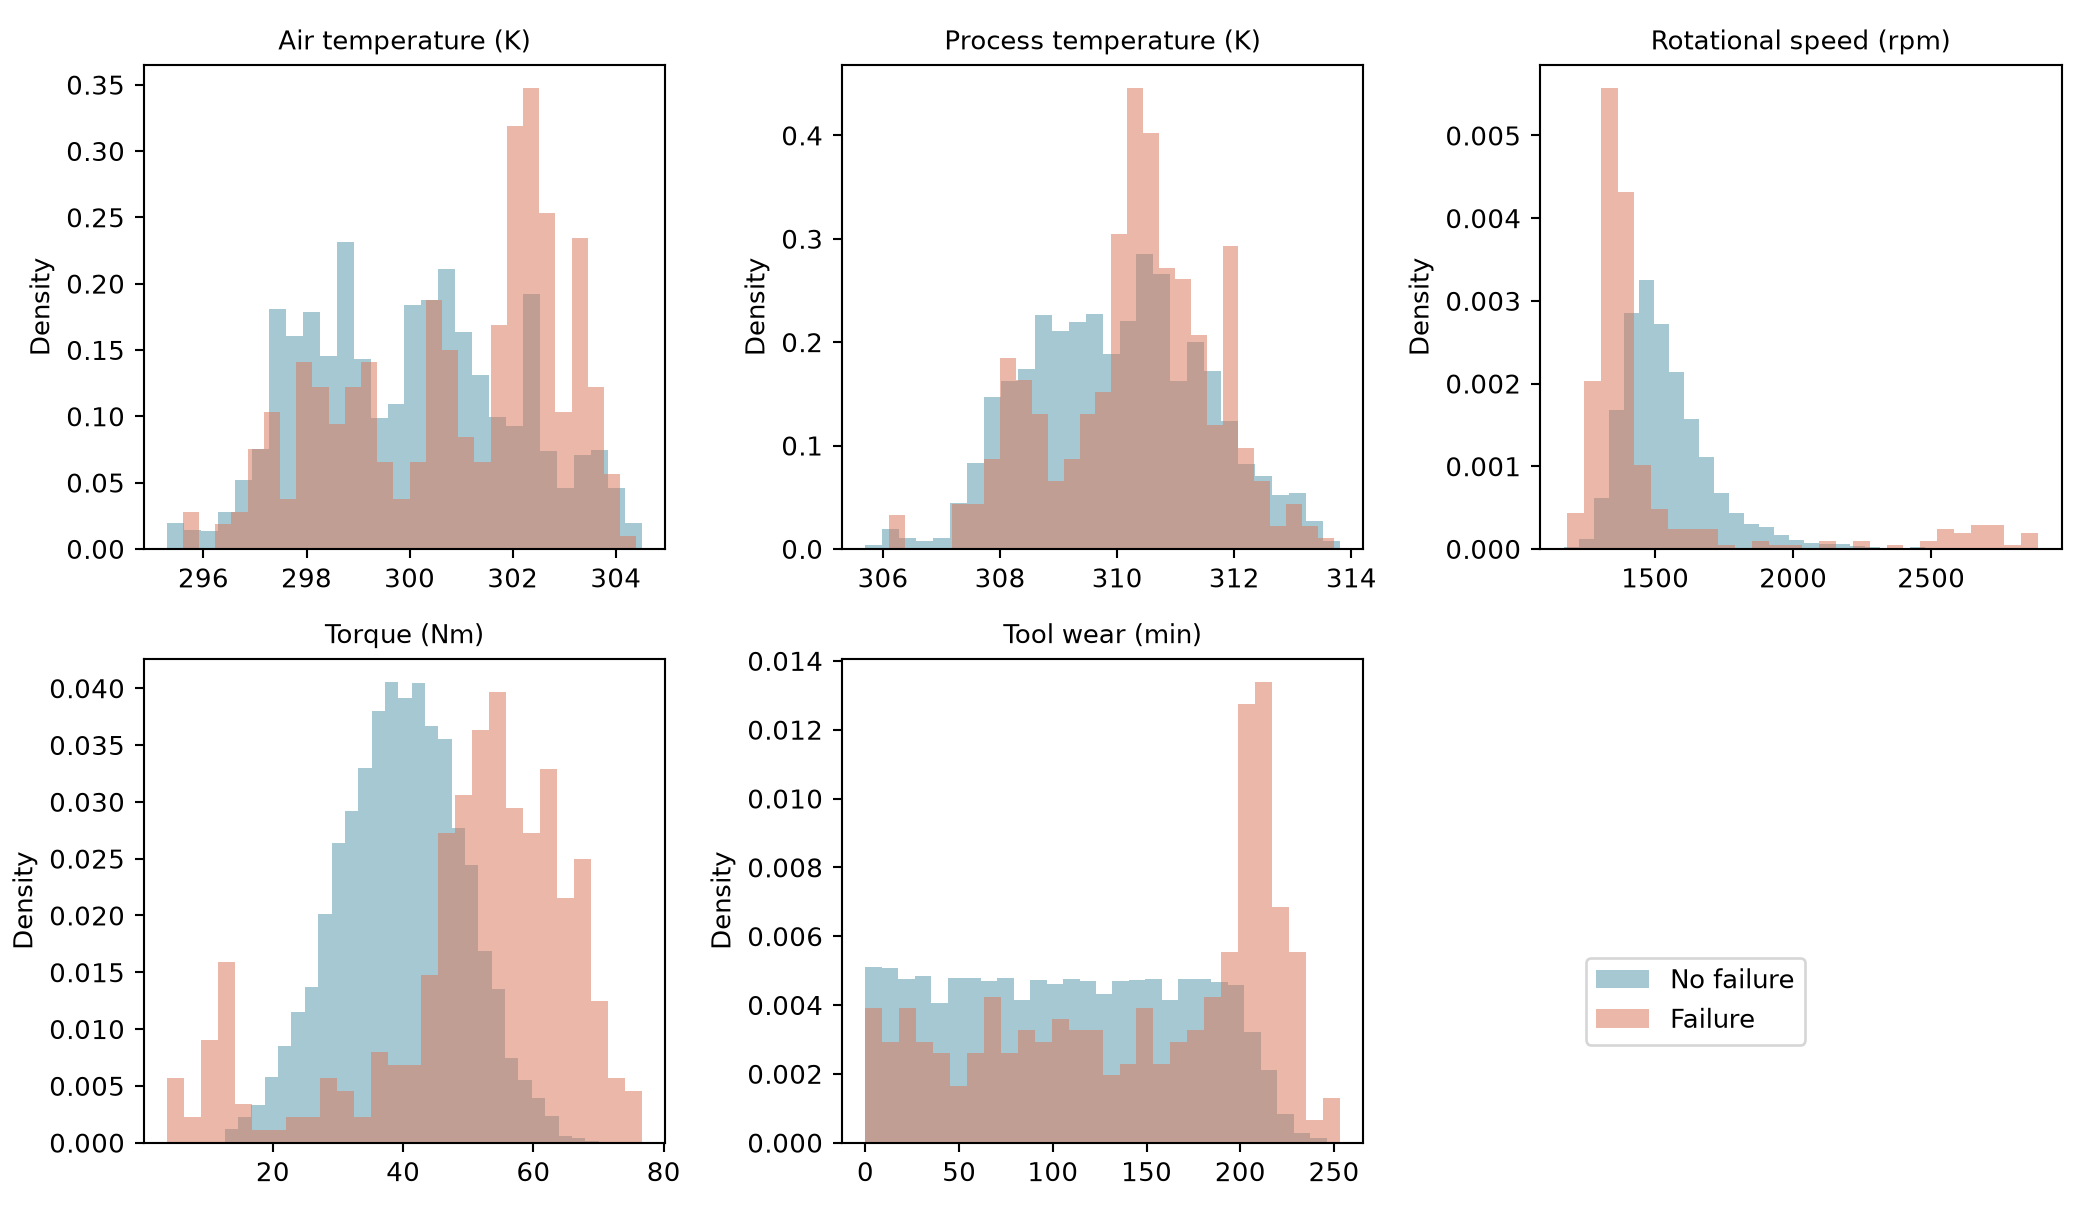
\includegraphics[width=.98\textwidth]{sensor_distributions.png}\caption{Phân phối các phép đo theo nhãn, dùng để khảo sát trước mô hình hóa.}\label{fig:sensors}\end{figure}

Các cột chế độ hỏng có số dương lần lượt là TWF 46, HDF 115, PWF 95, OSF 98 và RNF 19. Tổng các số này không nhất thiết bằng 339 do một bản ghi có thể thuộc nhiều chế độ. Chúng chỉ được dùng để mô tả bộ dữ liệu; mô hình không nhận chúng làm đầu vào. Việc giữ ranh giới này cũng làm cho đánh giá ngoại tuyến nhất quán với sáu trường mà API nhận.

\begin{figure}[H]\centering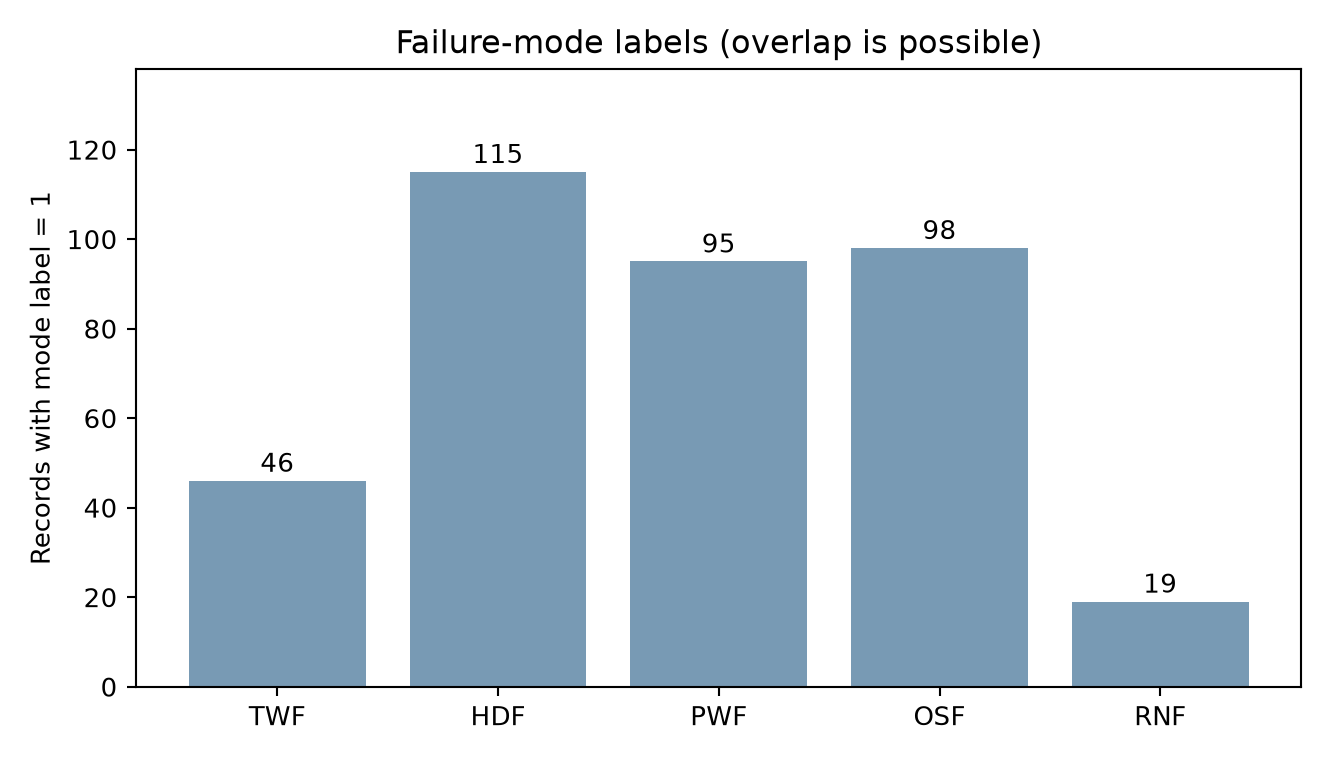
\includegraphics[width=.82\textwidth]{failure_modes.png}\caption{Số bản ghi dương theo từng cột chế độ hỏng; các nhóm có thể chồng lấn.}\label{fig:modes}\end{figure}

\section{Thiết kế phép chia tập}
Đầu tiên nhóm tách 20\% bản ghi làm test, có phân tầng theo nhãn. Sau đó lấy 20\% của phần 80\% còn lại làm validation. Kết quả là tỷ lệ 64/16/20, seed 42. Bảng~\ref{tab:split} cho thấy tỷ lệ hỏng được duy trì gần như nhau. Test được giữ riêng cho đến khi chọn xong mô hình và ngưỡng.

\begin{table}[H]\centering\caption{Phân chia dữ liệu dùng trong thực nghiệm}\label{tab:split}
\begin{tabular}{lrrr}\toprule Tập & Số bản ghi & Số hỏng & Tỷ lệ hỏng\\\midrule
Train & 6.400 & 217 & 3,39\% \\
Validation & 1.600 & 54 & 3,38\% \\
Test & 2.000 & 68 & 3,40\% \\
\bottomrule

\end{tabular}\end{table}

Không có khóa thiết bị lặp lại để thực hiện chia theo máy, và không có chuỗi thời gian để chia theo mốc. Do đó đánh giá này là nội bộ trên tập tĩnh. Nếu có dữ liệu thực tế, thiết kế phù hợp hơn sẽ tách theo thiết bị hoặc theo thời gian triển khai, tránh để những trạng thái rất gần nhau của một máy xuất hiện cả ở train và test. Cần xác định rõ ``thời điểm dự báo'' và khoảng thời gian trước hỏng trước khi gọi kết quả là cảnh báo sớm.


\chapter{Thiết kế hệ thống}
\section{Yêu cầu chức năng và phi chức năng}
Hệ thống cần nhận dữ liệu gốc có thể kiểm tra được, huấn luyện ba ứng viên theo cùng phép chia, chọn mô hình bằng validation, trả về xác suất hỏng qua HTTP và tạo báo cáo khi phân phối đầu vào thay đổi. Các đầu ra cần truy vết đến cấu hình, mã nguồn và tệp dữ liệu. Nhóm cũng đặt yêu cầu một người khác có thể cài phụ thuộc và chạy lại trên máy cá nhân; thiếu mô hình hoặc schema đầu vào sai phải tạo lỗi rõ ràng thay vì trả về dự đoán giả.

Về mặt phi chức năng, đây là bản mẫu học phần nên không đặt mục tiêu số yêu cầu mỗi giây hay độ trễ dịch vụ sản xuất. Tính tái tạo được kiểm tra qua seed, khóa phụ thuộc ở mức phù hợp, dấu băm dữ liệu và lệnh chạy pipeline. Tính quan sát được thể hiện qua MLflow, tệp metric và báo cáo giám sát. Tính di động được hỗ trợ bởi Python package và Docker image CPU. Tính an toàn dữ liệu ở đây tập trung vào xác thực trường đầu vào và tránh rò rỉ nhãn; hệ thống chưa có xác thực người dùng hoặc chính sách lưu trữ dữ liệu công nghiệp.

\section{Sơ đồ tổng thể}
Hình~\ref{fig:arch} mô tả đường dữ liệu và đường phục vụ. Bước \src{download} tạo CSV thô; bước \src{train} tạo mô hình, số liệu và tập tham chiếu. MLflow ghi từng lần huấn luyện vào SQLite cục bộ. API nạp cùng mô hình đã được chọn, còn công cụ monitor dùng \src{reference.csv} và một lô mới để xuất JSON trạng thái. CI chạy kiểm thử mã, độc lập với việc huấn luyện lại toàn bộ bộ dữ liệu.

\begin{figure}[H]\centering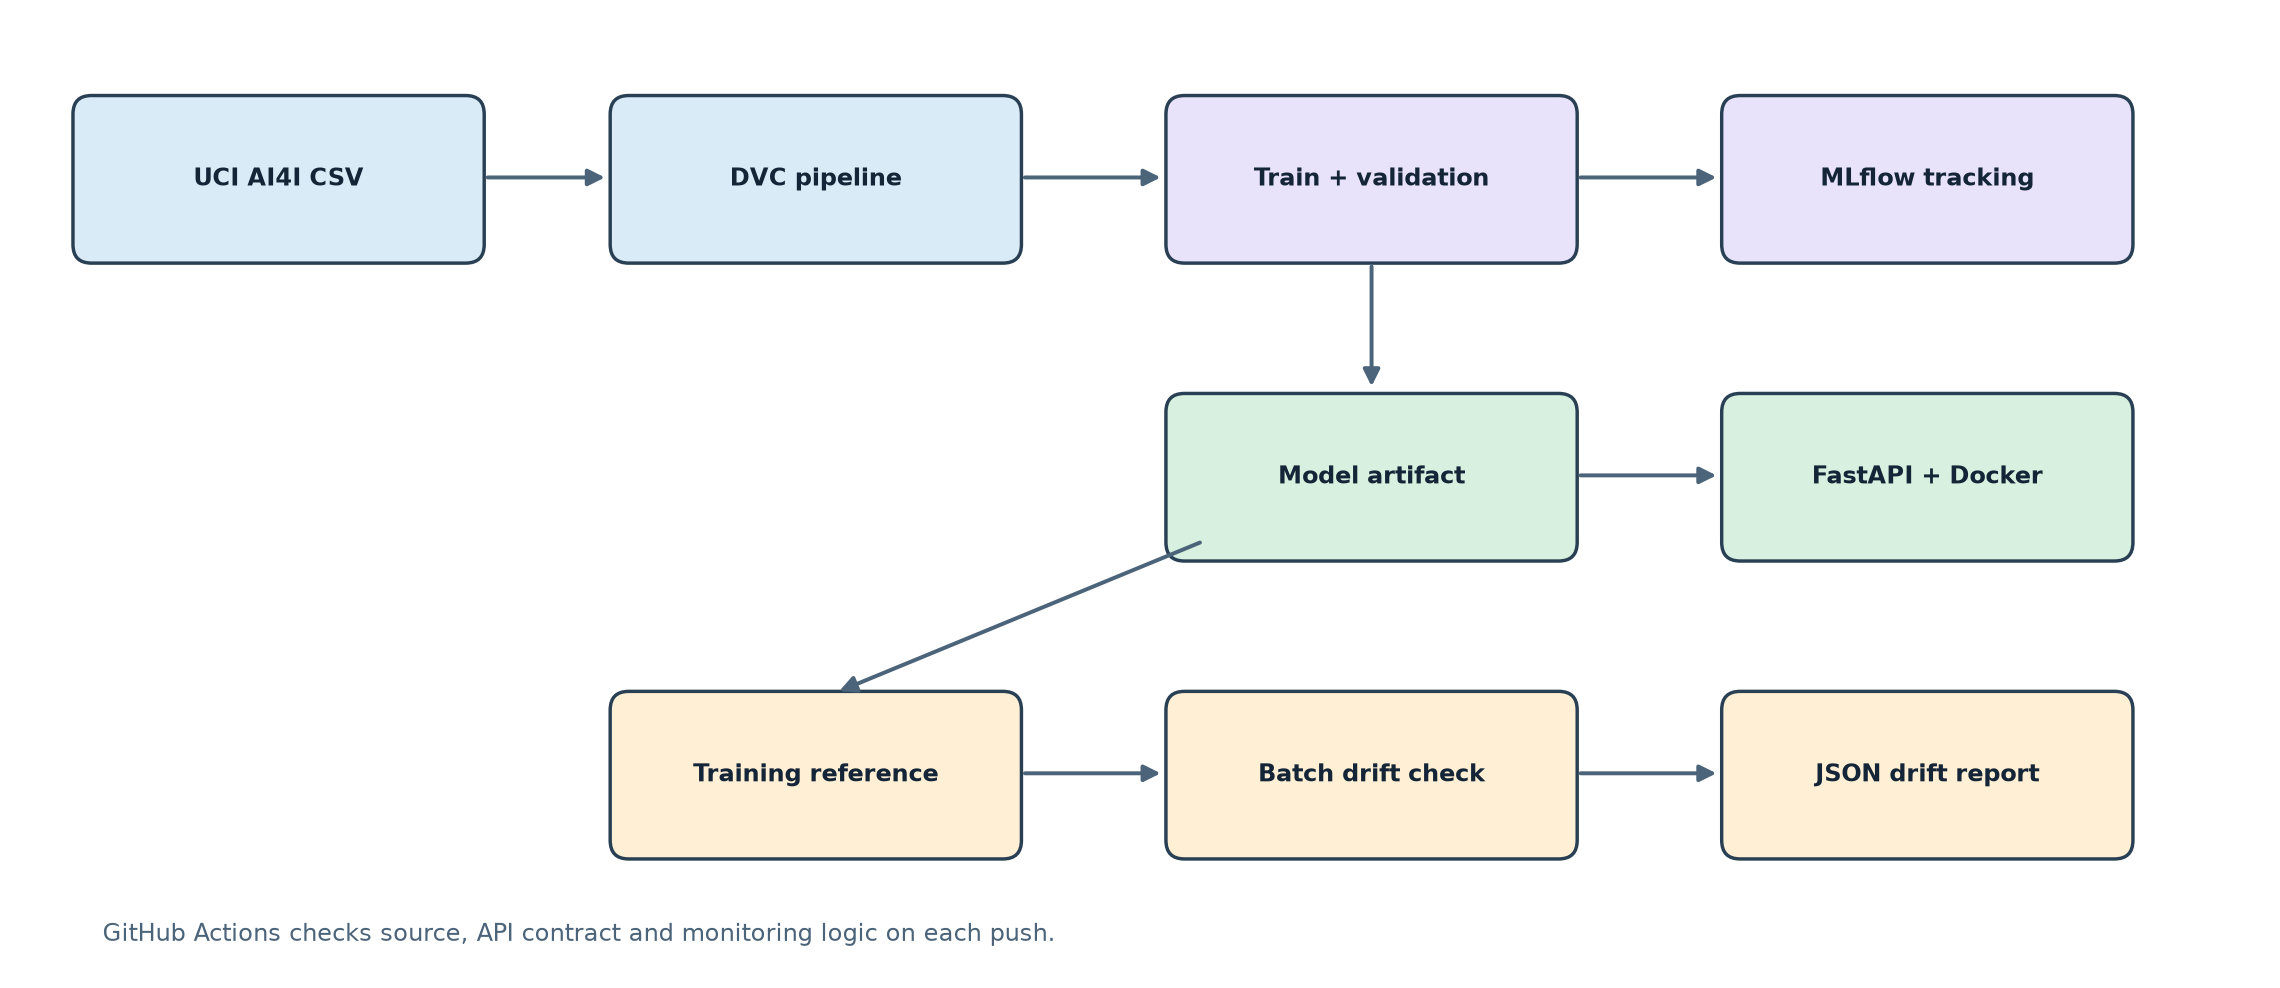
\includegraphics[width=.98\textwidth]{architecture.png}\caption{Kiến trúc triển khai của dự án. Mũi tên chỉ luồng dữ liệu hoặc hiện vật.}\label{fig:arch}\end{figure}

\section{Ranh giới các thành phần}
\src{src/predictive_maintenance/data.py} chịu trách nhiệm tải dữ liệu. \src{features.py} là hợp đồng schema huấn luyện. \src{splits.py} quy định một phép chia tập dùng chung. \src{train.py} định nghĩa tiền xử lý, ứng viên, đánh giá và xuất hiện vật. \src{api.py} nạp mô hình và nhận một bản ghi JSON; \src{monitor.py} nhận lô CSV và so sánh phân phối; \src{simulate.py} tạo dữ liệu để thử cảnh báo; \src{report.py} tổng hợp bằng chứng từ hiện vật. Phân công theo chức năng này giúp thay đổi một phần mà vẫn có thể xác định tác động đến phần khác.

Đầu ra của bước train gồm \src{model.joblib}, \src{metrics.json}, \src{reference.csv}. \src{model.joblib} chứa cả pipeline tiền xử lý, bộ phân loại, ngưỡng xác suất và danh sách sáu thuộc tính. API dùng đúng bundle này, tránh tái tạo bằng tay tiền xử lý khi triển khai. \src{metrics.json} giữ kết quả của từng ứng viên trên validation và một kết quả test của mô hình được chọn. \src{reference.csv} chỉ chứa thuộc tính của tập train, không chứa nhãn hoặc test; đây là đường chuẩn cho giám sát.

\section{Luồng huấn luyện và luồng suy luận}
Luồng huấn luyện bắt đầu từ CSV đã xác thực, chọn sáu thuộc tính, chia tập, khớp ba pipeline, ghi MLflow, chọn AP cao nhất, đánh giá test và lưu bundle. Mỗi ứng viên có cùng cách mã hóa \src{Type} và chuẩn hóa năm biến số. Đặt tiền xử lý trong pipeline làm giảm nguy cơ sử dụng thống kê từ validation hoặc test. Nếu thay đổi danh sách thuộc tính, hiện vật mô hình và hợp đồng API phải được cập nhật cùng nhau.

Luồng suy luận nhận JSON có sáu trường. Pydantic kiểm tra kiểu và miền giá trị cơ bản: \src{type} thuộc L/M/H, các nhiệt độ và tốc độ dương, mô-men xoắn và hao mòn không âm. API ánh xạ tên thân thiện của JSON sang tên cột CSV, gọi \src{predict_proba}, so sánh với ngưỡng được lưu trong bundle rồi trả về xác suất, cờ cảnh báo và ngưỡng. Điểm \src{/health} thử nạp mô hình; nếu tệp thiếu, nó trả 503. Kiểm tra này cho biết dịch vụ có nạp được hiện vật, chưa đo tính đúng đắn hay độ tươi của dữ liệu.

\section{Luồng giám sát và phản hồi}
Công cụ giám sát đọc một lô CSV, kiểm tra đủ sáu cột và số dòng tối thiểu. Với \src{Type}, nó so sánh tần suất ba giá trị; với từng biến số, nó loại giá trị không phải số hữu hạn trước phép thử KS và ghi lại số hàng lỗi. Kết quả trả về \src{ok} nếu không có thuộc tính lệch và không có lỗi chất lượng; còn lại trả \src{alert}. Cấu trúc JSON chứa chi tiết từng thuộc tính, giúp người vận hành biết cảnh báo do biến nào và do độ lệch hay do dữ liệu không hợp lệ.

Giám sát đầu vào chỉ là bước đầu của vòng phản hồi. Nếu có nhãn hỏng thật được xác nhận muộn hơn, người vận hành có thể nối dự đoán với nhãn để tính precision, recall, tỷ lệ cảnh báo và hiệu chuẩn theo thời gian. Bản mẫu chưa thực hiện bước này vì các lô demo không mô phỏng quy trình gán nhãn trễ. Một cảnh báo drift cũng không nên tự động kích hoạt huấn luyện lại: trước tiên cần kiểm tra lỗi thu thập, thay đổi thiết bị, tính hợp lệ của nhãn và kết quả trên một tập đánh giá mới.

\section{Quyết định triển khai và đánh đổi}
DVC được chọn để trình bày phụ thuộc giữa hai giai đoạn, nhưng cache chỉ có trên máy chạy, chưa cấu hình remote. MLflow dùng SQLite cục bộ, thuận tiện cho bài tập một máy nhưng không phải hạ tầng cộng tác nhiều người. Docker image chỉ cài phần phụ thuộc cần để phục vụ API, trong khi khâu huấn luyện chạy ngoài image. Cấu hình này giảm kích thước và thời gian dựng image, đồng thời đòi hỏi mô hình phải được tạo trước và gắn vào container ở chế độ chỉ đọc. Những đánh đổi này là quyết định có chủ đích theo phạm vi học phần.


\chapter{Phương pháp xây dựng mô hình}
\section{Chuẩn bị đầu vào}
Nhóm chỉ nhận sáu cột trong Bảng~\ref{tab:features} vào $X$. \src{Type} được one-hot encoding; năm biến số được StandardScaler khớp trên train. Cùng một \src{ColumnTransformer} được đặt trước từng bộ phân loại. Mặc dù cây quyết định thường không đòi hỏi chuẩn hóa biến số, cách thống nhất tiền xử lý khiến so sánh ba ứng viên dùng đúng cùng ma trận thuộc tính và tránh nhánh xử lý riêng cho từng mô hình. Nó không có nghĩa chuẩn hóa làm XGBoost mạnh hơn; báo cáo chưa thực hiện thí nghiệm cắt bỏ bước này.

Hàm chọn thuộc tính từ chối dữ liệu thiếu ở các cột bắt buộc, loại \src{Type} lạ và nhãn ngoài $\{0,1\}$. Sau phép chia, bộ tiền xử lý chỉ được \src{fit} cùng mô hình trên tập train. Bất kỳ thống kê trung bình, độ lệch chuẩn hay mã hóa danh mục nào cũng không được tính từ test. Đây là điểm cần kiểm tra khi chuyển mã từ notebook sang dịch vụ, vì hai đường tiền xử lý không đồng nhất có thể tạo dự đoán khác nhau dù dùng cùng hệ số mô hình.

\section{Các mô hình ứng viên và cấu hình}
Ba ứng viên được định nghĩa tường minh trong \src{train.py}. Logistic Regression có tối đa 1.000 vòng lặp và \src{class_weight="balanced"}. Random Forest có 200 cây, \src{min_samples_leaf=2} và \src{class_weight="balanced_subsample"}. XGBoost có 250 cây, \src{max_depth=4}, \src{learning_rate=0.05}, \src{subsample=0.9}, \src{colsample_bytree=0.9} và hàm đánh giá nội bộ \src{logloss}. Cả ba dùng seed 42 ở các chỗ liên quan và chạy trên CPU.

Đây là một tập cấu hình cố định nhằm so sánh quy trình, không phải tìm kiếm rộng để đạt điểm tối đa. XGBoost không dùng trọng số lớp trong triển khai hiện tại; điều đó cần được nhớ khi giải thích kết quả giữa các mô hình. Nếu tiếp tục tối ưu, nên tách một quy trình tìm kiếm siêu tham số trên train/validation, giới hạn ngân sách thử nghiệm và chỉ kiểm tra test sau khi chốt toàn bộ lựa chọn. Việc lặp lại lựa chọn nhiều lần theo test sẽ làm ước lượng test quá lạc quan.

\section{Quy tắc lựa chọn}
Với từng ứng viên $m$, chương trình tính xác suất trên validation và tính $AP_m$. Mô hình có AP lớn nhất được chọn. Việc chọn theo AP phản ánh mong muốn xếp các trường hợp hỏng lên trước trong dữ liệu có tỷ lệ dương thấp. Sau đó, với xác suất validation của mỗi mô hình, chương trình quét 91 ngưỡng cách đều từ 0,05 đến 0,95 và chọn ngưỡng cho $F_2$ cao nhất. \src{numpy.argmax} lấy vị trí đầu tiên khi có hòa điểm, tức là ngưỡng thấp hơn trong dãy tăng dần. Ngưỡng của ứng viên được chọn đi cùng hiện vật mô hình.

\begin{equation}
m^*=\underset{m\in\{LR,RF,XGB\}}{\arg\max}\,AP_m^{(val)},\qquad
t^*=\underset{t\in\{0.05,0.06,\ldots,0.95\}}{\arg\max}\,F_2^{(val)}(m^*,t).
\end{equation}

Quy tắc này tách hai mục tiêu: chọn thuật toán xếp hạng tốt và chọn điểm vận hành ưu tiên recall. Nó không đưa ra xác suất đã hiệu chuẩn cho quyết định chi phí. Ngưỡng 0,15 là kết quả trên validation của dataset hiện tại; không nên sao chép nguyên xi sang máy thật. Để quyết định ngưỡng thực tế, cần đánh giá hiệu chuẩn, tần suất cảnh báo, chi phí kiểm tra và chi phí bỏ sót cùng chuyên gia bảo trì.

\section{Các chỉ số đánh giá}
Sau khi chọn mô hình và ngưỡng, chương trình tính AP, ROC-AUC, precision, recall, $F_1$, $F_2$ và bốn ô ma trận nhầm lẫn trên test. AP và ROC-AUC sử dụng xác suất chưa nhị phân hóa; các chỉ số còn lại dùng $p\geq t^*$. Việc báo cả hai loại số đo tránh diễn giải sai rằng AP là precision tại ngưỡng được chọn. Bảng validation cũng ghi precision, recall và $F_2$ tại ngưỡng riêng của từng ứng viên, giúp nhìn mức đánh đổi khi chuyển từ khả năng xếp hạng sang cảnh báo cụ thể.

Số lượng dương ở test chỉ là 68, vì vậy các chỉ số theo lớp hỏng chịu biến động nếu thay đổi phép chia. Báo cáo không ước lượng khoảng tin cậy hay đánh giá trên nhiều seed, nên không thể khẳng định chênh lệch nhỏ giữa các cấu hình là bền vững. Tuy nhiên, so sánh validation của ba mô hình cho thấy khác biệt AP khá rõ trong chính phép chia đã định. Kết quả test được trình bày như bằng chứng thực nghiệm có giới hạn, không phải bảo đảm vận hành.

\section{Lưu hiện vật và tái hiện dự đoán}
Bundle \src{model.joblib} chứa đối tượng pipeline đã khớp, ngưỡng và danh sách đặc trưng. \src{metrics.json} là tóm tắt có cấu trúc; nó ghi toàn bộ bảng so sánh validation và kết quả test. MLflow lưu tham số, các metric theo tiền tố \src{validation_} và các metric test gắn với run mô hình được chọn; mô hình và tệp metric cũng được đính kèm run này. Tệp \src{reference.csv} được xuất từ \emph{train} sau chia tập, giữ nguyên sáu cột đầu vào để monitor đọc lại.

Chương trình tạo bằng chứng của báo cáo kiểm tra dữ liệu và tính lại dự đoán từ bundle trước khi dựng biểu đồ. Cơ chế này hữu ích vì sao chép số liệu thủ công từ nhiều lần chạy dễ gây nhầm lẫn. Dù vậy, các hiện vật nhị phân vẫn phụ thuộc phiên bản thư viện; dự án ghi phiên bản đã chạy và Docker API dùng tập phụ thuộc tương thích. Với hệ thống lâu dài, cần một kho hiện vật có phiên bản, kiểm tra tương thích khi nâng cấp thư viện và quy trình phê duyệt mô hình.


\chapter{Hiện thực quy trình MLOps}
\section{Cấu trúc repository và môi trường}
Repository công khai của nhóm ở \url{https://github.com/kienluongzero-hue/MLops}. Mã chính nằm trong package \src{src/predictive_maintenance}; \src{tests} chứa kiểm thử; \src{reports} lưu bằng chứng và hình; \src{latex-report} chứa nguồn báo cáo. \src{pyproject.toml} khai báo phần phụ thuộc cơ bản, phần thêm cho huấn luyện, báo cáo và phát triển. Trong lần chạy được báo cáo, môi trường có Python 3.13.12, scikit-learn 1.9.1, XGBoost 3.4.1 và MLflow 3.18.0. Những phiên bản này ghi nhận trạng thái thực nghiệm, không có nghĩa mọi bản vá tương lai đều tái tạo bit-for-bit cùng kết quả.

\section{DVC: mô tả quan hệ giữa các bước}
\src{dvc.yaml} có hai stage. \src{download} gọi mô-đun tải CSV và xuất \src{data/raw/ai4i2020.csv}. \src{train} phụ thuộc CSV, mã huấn luyện, mã đặc trưng, mã chia tập và \src{pyproject.toml}; nó xuất mô hình, metric và tập tham chiếu. DVC dùng trạng thái phụ thuộc và khóa trong \src{dvc.lock} để biết khi nào cần chạy lại \cite{dvc}. Ví dụ, đổi định nghĩa tiền xử lý làm stage train lỗi thời, nhưng không buộc tải lại dữ liệu nếu CSV và bước download không đổi.

\begin{lstlisting}[language={},caption={Hai stage chính trong cấu hình DVC},label={lst:dvc}]
stages:
  download:
    cmd: python -m predictive_maintenance.data
    outs: [data/raw/ai4i2020.csv]
  train:
    cmd: python -m predictive_maintenance.train
    deps: [data/raw/ai4i2020.csv,
           src/predictive_maintenance/train.py,
           src/predictive_maintenance/features.py,
           src/predictive_maintenance/splits.py,
           pyproject.toml]
    outs: [artifacts/model.joblib, artifacts/metrics.json,
           artifacts/reference.csv]
\end{lstlisting}
Listing~\ref{lst:dvc} rút gọn cấu hình để thể hiện phụ thuộc, không phải bản thay thế cho tệp trong repository. Hiện dự án chưa có DVC remote. Người clone repository phải chạy stage download từ nguồn UCI và train trên máy mình; họ không thể \src{dvc pull} mô hình từ một kho hiện vật nhóm. SHA-256 của dữ liệu gốc hỗ trợ phát hiện sai khác nếu URL nguồn trả nội dung khác.

\section{MLflow: dấu vết thí nghiệm}
Trước khi chạy các ứng viên, chương trình đặt tracking URI là \src{sqlite:///mlflow.db} và chọn experiment \src{predictive-maintenance-ai4i}. Mỗi mô hình được khớp trong một MLflow run tên tương ứng. Run lưu tên mô hình, seed, số bản ghi train và validation, ngưỡng đã chọn, các metric validation. Sau khi chọn XGBoost, chương trình ghi thêm metric test và đính kèm mô hình đã xuất vào run được chọn. Giao diện MLflow cho phép so sánh các run và xem cùng một định nghĩa chỉ số \cite{mlflow}.

SQLite cục bộ là lựa chọn đơn giản cho một máy; tệp database nằm ngoài Git. Khi nhiều thành viên cần cùng một lịch sử, nhóm phải dùng tracking server có kho backend và artifact chung, kiểm soát quyền truy cập và sao lưu. Cũng cần quy ước tên run, tag phiên bản dữ liệu và mã Git nếu quy mô thử nghiệm tăng. Báo cáo hiện tại không tuyên bố đã có model registry hay quy trình chuyển trạng thái mô hình sang production.

\section{FastAPI và hợp đồng suy luận}
Ứng dụng định nghĩa \src{GET /health} và \src{POST /predict}. Đầu vào POST là một đối tượng gồm \src{type}, \src{air_temperature}, \src{process_temperature}, \src{rotational_speed}, \src{torque}, \src{tool_wear}. Pydantic từ chối thiếu trường, sai kiểu hoặc giá trị nằm ngoài miền kiểm tra cơ bản. Sau khi ánh xạ sang tên cột huấn luyện, API trả \src{failure_probability}, \src{predicted_failure} và \src{threshold}. Tải mô hình có cache trong quá trình chạy để không đọc tệp cho mọi yêu cầu.

\begin{lstlisting}[language={},caption={Ví dụ yêu cầu và phản hồi API},label={lst:api}]
POST /predict
{"type":"L","air_temperature":298.1,
 "process_temperature":308.6,"rotational_speed":1551,
 "torque":42.8,"tool_wear":0}

{"failure_probability": <gia tri thuc>,
 "predicted_failure": <true hoac false>,
 "threshold": 0.15}
\end{lstlisting}
Listing~\ref{lst:api} cố ý để trống xác suất cụ thể vì đó là kết quả phụ thuộc hiện vật mô hình và không được ghi nhận như một số liệu cố định của báo cáo. Trường ngưỡng thực tế trong JSON có thể hiển thị gần 0,15 do biểu diễn số thực dấu phẩy động. Xác thực hiện tại chỉ kiểm tra miền giá trị rộng, chưa kiểm tra giới hạn vật lý phù hợp từng thiết bị; nếu áp dụng thực tế, hợp đồng cần giới hạn và đơn vị đo được thống nhất với hệ thống thu thập.

\section{Docker và đóng gói dịch vụ}
Dockerfile bắt đầu từ \src{python:3.13-slim}, sao chép cấu hình phụ thuộc và mã nguồn, cài gói cho API, rồi chạy Uvicorn trên cổng 8000 \cite{docker}. Tệp yêu cầu riêng cho API tránh cài MLflow, DVC và công cụ vẽ hình vào image phục vụ. Mô hình không được đóng sẵn trong image; khi chạy container, thư mục \src{artifacts} từ máy chủ được gắn vào \src{/app/artifacts} ở chế độ chỉ đọc. Điều này cho phép thay hiện vật mô hình mà không sửa mã image, nhưng người triển khai phải bảo đảm mô hình được sinh từ phiên bản package tương thích và được kiểm tra trước khi gắn.

\begin{lstlisting}[language={},caption={Dựng và chạy API trong Docker},label={lst:docker}]
docker build -t predictive-maintenance-api .
docker run --rm -p 8000:8000 \
  -v "${PWD}/artifacts:/app/artifacts:ro" \
  predictive-maintenance-api
\end{lstlisting}
Lệnh gắn volume trong Listing~\ref{lst:docker} mang tính minh họa cho shell có cú pháp tương ứng; README có phiên bản PowerShell một dòng. Container trả 503 ở \src{/health} nếu chưa tìm thấy hiện vật. Docker tạo môi trường chạy đồng nhất hơn giữa máy, nhưng không bảo đảm chất lượng mô hình khi dữ liệu triển khai khác dữ liệu phát triển.

\section{Kiểm thử tự động và bằng chứng}
Workflow GitHub Actions chạy khi push hoặc mở pull request. Nó checkout mã, chuẩn bị Python 3.12, cài gói với phần \src{dev} rồi chạy \src{pytest} \cite{actions}. Đây là bước kiểm soát hồi quy ở mức mã, không chạy toàn bộ huấn luyện vì pipeline còn phụ thuộc dữ liệu tải ngoài và thời gian huấn luyện. Kiểm thử API và các hàm xử lý giúp phát hiện lỗi schema và thay đổi hành vi cơ bản. Trong một hệ thống triển khai thật, cần thêm kiểm thử trên dữ liệu đại diện, kiểm tra chất lượng mô hình theo ngưỡng chấp nhận và thử image trong môi trường gần production; các gợi ý này phù hợp với quan điểm về kiểm thử hệ thống ML \cite{breck2017}.

\src{python -m predictive_maintenance.report} tạo \src{reports/evidence.json}, \src{evidence.md} và hai hình về kết quả mô hình, giám sát. Chương trình đối chiếu kết quả từ bundle với tệp metric, giúp phát hiện nếu một tệp bị thay mà tệp kia chưa cập nhật. \src{latex-report/generate_assets.py} tạo các bảng và hình bổ sung trực tiếp từ cùng hiện vật. Cả hai bước là công cụ lập báo cáo, không thay thế kiểm thử độc lập của mô hình.


\chapter{Thực nghiệm, kết quả và thảo luận}
\section{Thiết lập thực nghiệm}
Thực nghiệm sử dụng CSV gốc của UCI đã xác thực dấu băm, phép chia stratified seed 42 và ba pipeline mô hình trong Chương 5. Train có 6.400 bản ghi, trong đó 217 hỏng; validation có 1.600 bản ghi, trong đó 54 hỏng; test có 2.000 bản ghi, trong đó 68 hỏng. Tỷ lệ dương gần như bằng nhau giữa ba tập. Tất cả số liệu so sánh mô hình được tính trên validation; chỉ mô hình và ngưỡng đã chọn được đánh giá trên test. Máy tính sử dụng Python 3.13.12 với các phiên bản thư viện ghi ở Chương 6.

Quy trình chạy là: tải dữ liệu, huấn luyện ba ứng viên, xuất bundle và metric, tạo hai lô giám sát, chạy monitor, rồi sinh bằng chứng báo cáo. Mọi hình trong chương này được tạo từ CSV hoặc hiện vật của chính quy trình đó. Số liệu làm tròn ba chữ số thập phân để trình bày; tệp JSON giữ giá trị đầy đủ. Do chỉ có một phép chia, kết quả không bao gồm độ lệch chuẩn trên nhiều seed hay khoảng tin cậy. Đây là một hạn chế khi diễn giải khác biệt nhỏ giữa các thuật toán.

\section{So sánh ba ứng viên trên validation}
\begin{table}[H]\centering\caption{So sánh mô hình trên tập validation; precision, recall và $F_2$ tại ngưỡng riêng của từng mô hình}\label{tab:validation}
\begin{tabular}{lrrrr}\toprule Mô hình & AP & Precision & Recall & $F_2$\\\midrule
Logistic Regression & 0,420 & 0,285 & 0,685 & 0,535 \\
Random Forest & 0,712 & 0,440 & 0,815 & 0,696 \\
XGBoost & 0,780 & 0,581 & 0,796 & 0,741 \\
\bottomrule

\end{tabular}\end{table}
Logistic Regression đạt AP 0,420; Random Forest đạt 0,712; XGBoost đạt 0,780. Chênh lệch giữa đường chuẩn tuyến tính và hai mô hình cây cho thấy các quan hệ phi tuyến hoặc tương tác có thể quan trọng trong dataset này. Không thể từ đó kết luận một thuật toán luôn tốt hơn trên dữ liệu công nghiệp khác. Trong cùng phép chia, XGBoost đứng đầu theo quy tắc AP đã định trước, nên được chọn. Precision 0,581 và recall 0,796 của XGBoost trên validation là tại ngưỡng 0,15; Random Forest dùng 0,21 và Logistic Regression dùng 0,74.

\begin{figure}[H]\centering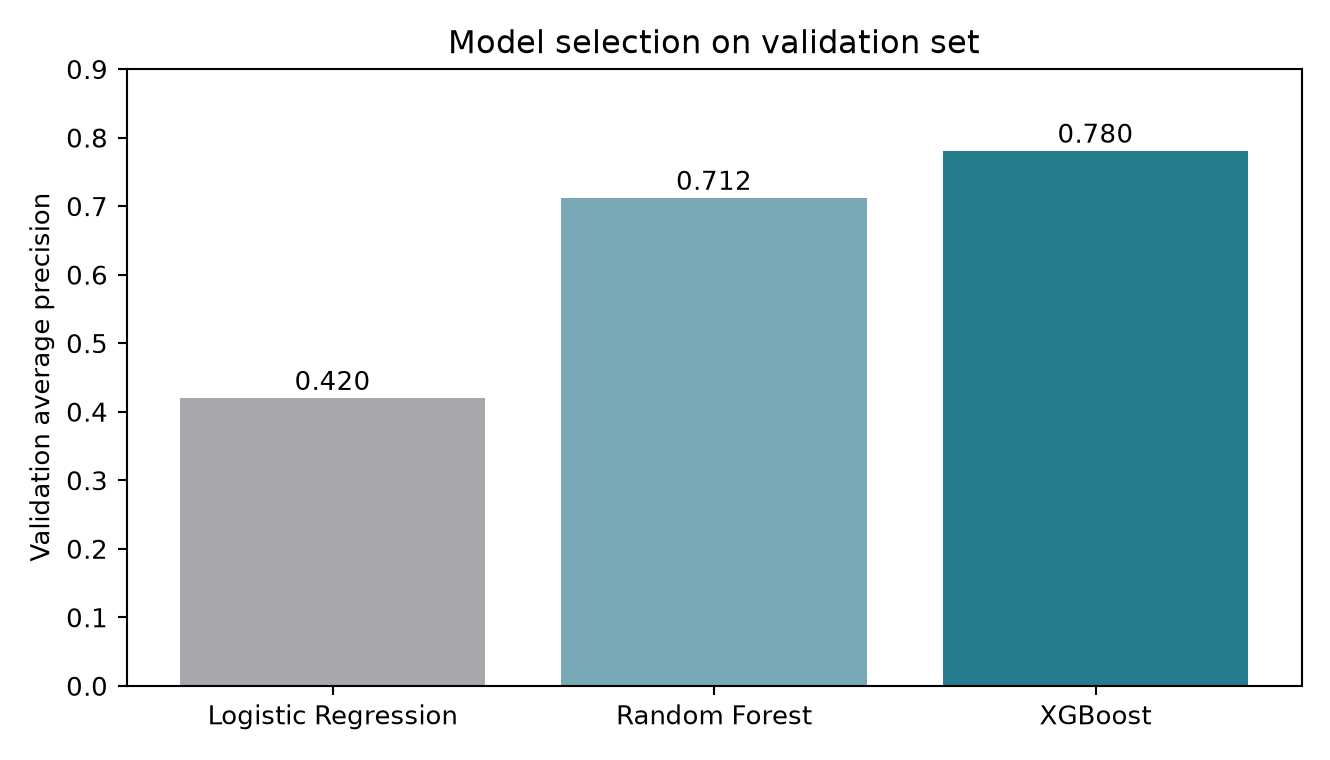
\includegraphics[width=.86\textwidth]{validation_comparison.png}\caption{Average precision của ba ứng viên trên validation.}\label{fig:validation}\end{figure}

AP là chỉ số xếp hạng tổng hợp, không nói trực tiếp số ca bỏ sót tại ngưỡng dùng trong dịch vụ. Vì vậy, bên cạnh AP, nhóm chọn ngưỡng bằng $F_2$ trên validation. Hình~\ref{fig:threshold} biểu diễn điểm $F_2$ của XGBoost theo dải 91 ngưỡng đã quét. Việc chỉ tối ưu trong một dải và bước 0,01 có nghĩa 0,15 là tối ưu \emph{trên lưới thử này}, không phải nghiệm liên tục tối ưu tuyệt đối. Nếu thay đổi mục tiêu ưu tiên hoặc chi phí cảnh báo sai, ngưỡng có thể thay đổi đáng kể.

\begin{figure}[H]\centering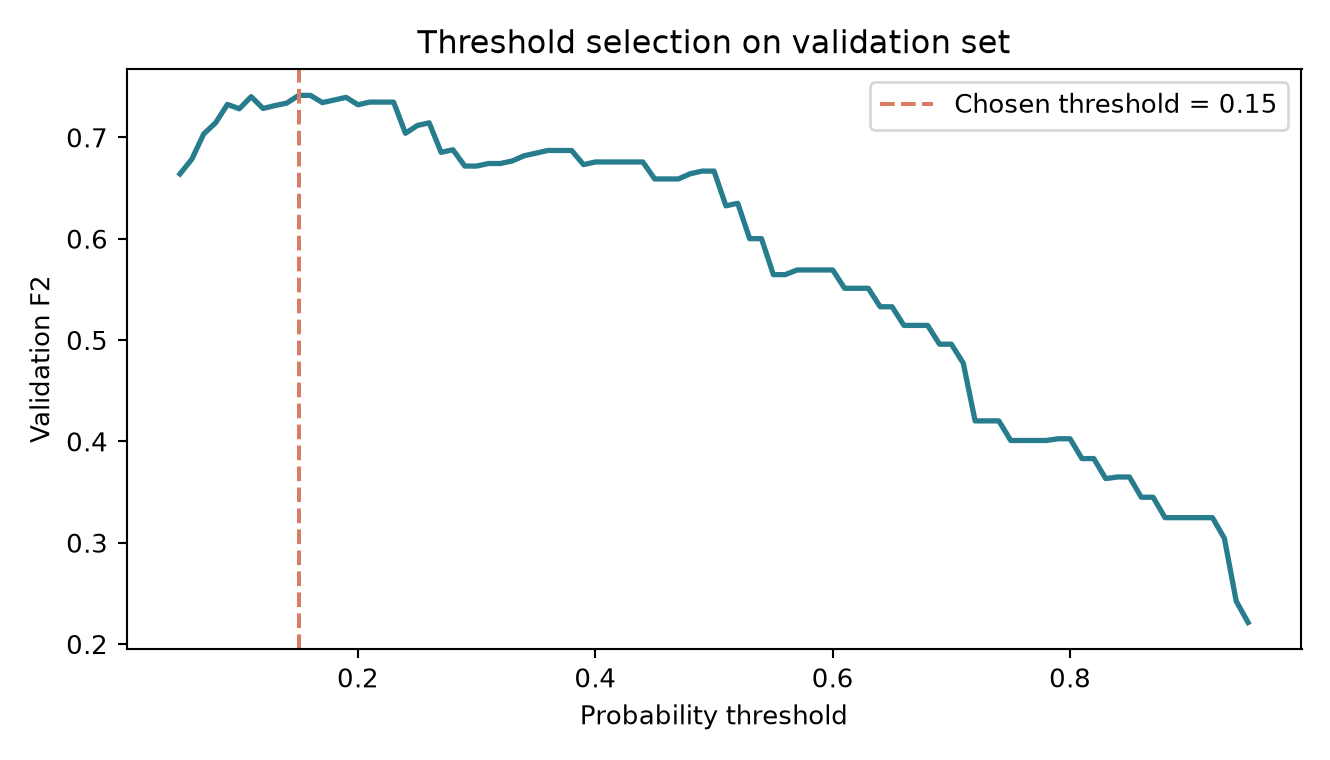
\includegraphics[width=.9\textwidth]{threshold_f2.png}\caption{Điểm $F_2$ trên validation theo ngưỡng của XGBoost; dấu đánh dấu chỉ ngưỡng được lưu.}\label{fig:threshold}\end{figure}

\section{Kết quả test của mô hình được chọn}
XGBoost với ngưỡng 0,15 đạt AP 0,825, ROC-AUC 0,974, precision 0,614, recall 0,794, $F_1$ 0,692 và $F_2$ 0,750 trên test. Cần phân biệt AP 0,825 với precision 0,614: AP đánh giá toàn dải ngưỡng, còn precision chỉ đánh giá các cảnh báo khi $p\geq0,15$. Chỉ số ROC-AUC cao cho thấy khả năng xếp thứ tự hai lớp trên tập test này, nhưng không trực tiếp phản ánh số cảnh báo sai trong lịch làm việc của nhân viên bảo trì.

\begin{table}[H]\centering\caption{Ma trận nhầm lẫn trên test, ngưỡng 0,15}\label{tab:confusion}
\begin{tabular}{lrr}\toprule Thực tế / dự đoán & Không hỏng & Hỏng\\\midrule
Không hỏng & 1.898 (TN) & 34 (FP)\\
Hỏng & 14 (FN) & 54 (TP)\\\bottomrule
\end{tabular}\end{table}
Trong 68 bản ghi hỏng, hệ thống phát hiện đúng 54 và bỏ sót 14. Trong 1.932 bản ghi không hỏng, 34 nhận cảnh báo sai. Tổng số cảnh báo là $54+34=88$, nên precision bằng $54/88\approx0,614$. Recall bằng $54/68\approx0,794$. Các phép tính này kiểm tra độc lập tính nhất quán của metric lưu trong JSON. Về vận hành, 34 cảnh báo sai có thể tạo thêm công việc kiểm tra; 14 ca bỏ sót vẫn là rủi ro. Không có dữ liệu chi phí, nên báo cáo không định giá tiền cho hai loại sai lầm.

\begin{figure}[H]\centering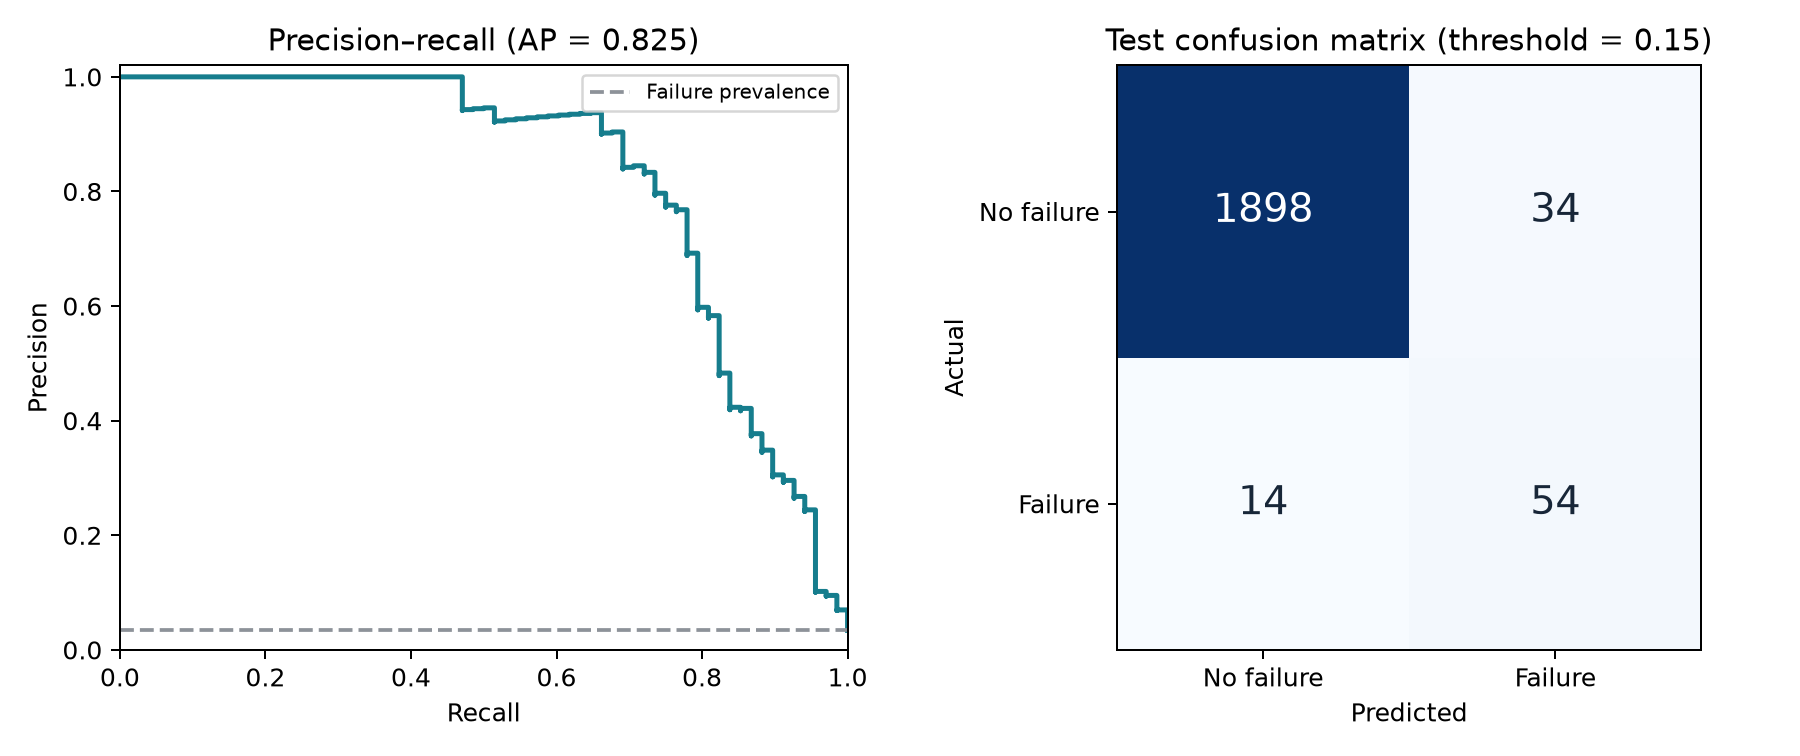
\includegraphics[width=.96\textwidth]{model_evaluation.png}\caption{Đường precision--recall và ma trận nhầm lẫn test của mô hình được chọn.}\label{fig:model_eval}\end{figure}

Độ chính xác tổng thể tính từ ma trận là $(1898+54)/2000=97,6\%$, nhưng con số này ít giúp đánh giá lớp hỏng khi tỷ lệ dương chỉ 3,39\%. Mốc luôn dự đoán không hỏng trên toàn bộ dữ liệu đã đạt accuracy 96,61\%. Chênh lệch giữa hai accuracy nhìn có vẻ nhỏ dù mô hình thật phát hiện 54 ca hỏng; đây là lý do báo cáo không dùng accuracy để chọn mô hình. Độ bao phủ của cảnh báo, precision và số FP/FN trực tiếp hơn cho quyết định kiểm tra.

\section{Diễn giải thuộc tính}
Hình~\ref{fig:importance} hiển thị mức độ quan trọng thuộc tính của XGBoost trong bundle đã huấn luyện. Đây là thống kê phụ thuộc cách xây dựng cây và cách thư viện tổng hợp đóng góp của các lần tách. Nó hữu ích để kiểm tra sơ bộ xem mô hình có dựa vào các biến cảm biến hợp lệ, nhưng không chứng minh rằng thay đổi một cảm biến sẽ gây ra hoặc ngăn hỏng máy. Các biến có tương quan có thể chia sẻ hoặc thay đổi thứ hạng độ quan trọng khi dữ liệu và seed thay đổi. Để giải thích từng cảnh báo với người vận hành, cần phương pháp diễn giải cục bộ và kiểm chứng với chuyên gia, chưa có trong bản mẫu.

\begin{figure}[H]\centering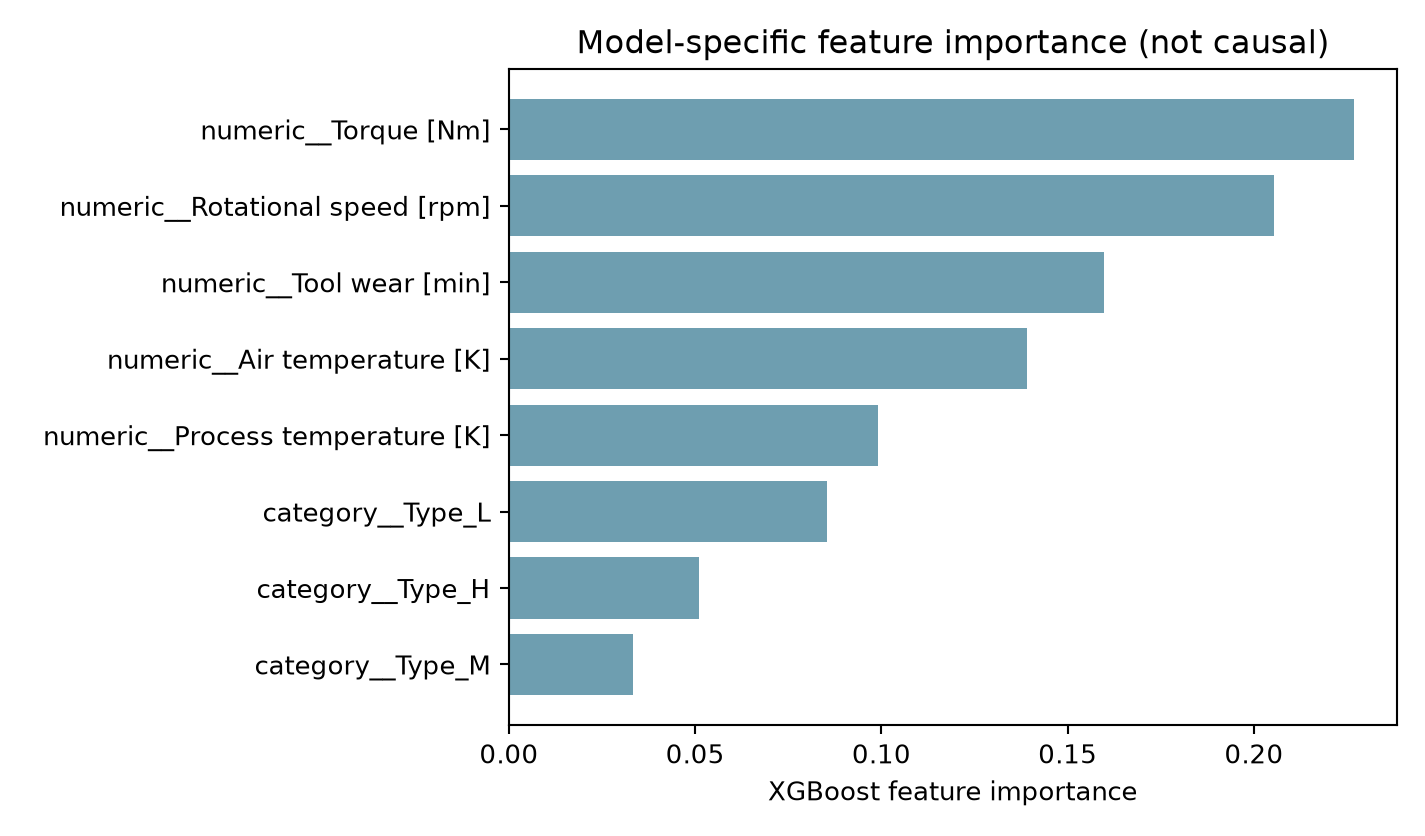
\includegraphics[width=.9\textwidth]{feature_importance.png}\caption{Độ quan trọng thuộc tính của XGBoost; chỉ diễn giải theo mô hình đã khớp.}\label{fig:importance}\end{figure}

\section{Phân tích lỗi sau đánh giá}
Sau khi cố định mô hình và ngưỡng, nhóm khảo sát các lỗi trên test để hiểu ý nghĩa của ma trận nhầm lẫn. Phân tích này chỉ mang tính mô tả hậu nghiệm: nó không được dùng để chọn lại thuật toán hoặc ngưỡng. Bảng~\ref{tab:subgroup} tách số dự đoán theo \src{Type}. Loại L có 38 bản ghi hỏng, phát hiện đúng 29 và bỏ sót 9; loại M có 25 bản ghi hỏng, phát hiện đúng 21 và bỏ sót 4; loại H có 5 bản ghi hỏng, phát hiện đúng 4 và bỏ sót 1. Các số dương của nhóm H rất ít, nên một trường hợp thêm hoặc bớt sẽ làm tỷ lệ thay đổi mạnh. Báo cáo vì vậy đưa số đếm thay vì khẳng định mô hình công bằng hoặc ổn định theo nhóm.

\begin{table}[H]\centering\caption{Kết quả test theo loại sản phẩm, chỉ để phân tích hậu nghiệm}\label{tab:subgroup}
\begin{tabular}{lrrrrr}\toprule Loại & Số dòng & Số hỏng & TP & FN & FP\\\midrule
L & 1.170 & 38 & 29 & 9 & 20 \\
M & 616 & 25 & 21 & 4 & 11 \\
H & 214 & 5 & 4 & 1 & 3 \\
\bottomrule

\end{tabular}\end{table}

Tổng TP, FN và FP theo ba nhóm phải lần lượt bằng 54, 14 và 34 như Bảng~\ref{tab:confusion}. Việc tự động kiểm tra tổng từ dự đoán của bundle trước khi sinh bảng giúp tránh lỗi sao chép thủ công. Không nên dùng bảng này để suy luận nguyên nhân khác biệt giữa các loại sản phẩm: mỗi nhóm có thể có phân phối tốc độ, mô-men hoặc hao mòn khác nhau, trong khi tập test không đủ lớn để đánh giá có điều chỉnh theo các biến đó.

\begin{table}[H]\centering\caption{Trung bình một số biến của bốn loại kết quả trên test}\label{tab:error-profiles}
\begin{tabular}{lrrrr}\toprule Nhóm & Số dòng & Xác suất & Torque (Nm) & Tool wear (min)\\\midrule
TP & 54 & 0,728 & 52,62 & 145,46 \\
FN & 14 & 0,051 & 40,65 & 183,64 \\
FP & 34 & 0,331 & 47,95 & 158,79 \\
TN & 1.898 & 0,006 & 39,41 & 106,54 \\
\bottomrule

\end{tabular}\end{table}

Bảng~\ref{tab:error-profiles} so sánh trung bình xác suất mà mô hình gán và hai biến vật lý theo bốn ô ma trận. Trong 14 âm giả, xác suất trung bình khoảng 0,051, thấp hơn ngưỡng 0,15; mức hao mòn trung bình của nhóm này khoảng 183,64 phút, cao hơn nhóm dương thật. Điều đó nhắc rằng một biến riêng lẻ cao không đủ để mô hình phát cảnh báo, vì dự đoán còn phụ thuộc các thuộc tính và tương tác khác. Trong 34 dương giả, xác suất trung bình khoảng 0,331; mô-men xoắn trung bình 47,95 Nm. Các trung bình này là mô tả của các tập con nhỏ, không phải quy tắc chẩn đoán hoặc giải thích nhân quả cho từng trường hợp.

Một bước phân tích tiếp theo nên mở từng bản ghi FN với thông tin thiết bị và thời điểm, hỏi chuyên gia liệu nhãn có chính xác, cảm biến có hoạt động bình thường và hành động kiểm tra nào đã xảy ra. Dữ liệu AI4I không cung cấp chuỗi bối cảnh đó. Việc chỉ dựa vào một biểu đồ độ quan trọng toàn cục để giải thích một âm giả cụ thể sẽ dễ dẫn đến kết luận quá mức. Nhóm giữ bảng lỗi ở mức thống kê và ghi rõ giới hạn này.

\section{Thử nghiệm giám sát dữ liệu đầu vào}
Tham chiếu của monitor là 6.400 bản ghi train. Hai lô thử nghiệm cùng có 500 bản ghi được lấy từ phần dữ liệu giữ lại. Lô bình thường giữ nguyên các phép đo; lô dịch chuyển được tạo có chủ đích bằng cộng 5 K vào nhiệt độ không khí, cộng 10 Nm vào mô-men xoắn và đặt 60\% bản ghi thành loại H. Như vậy thí nghiệm kiểm tra khả năng phát hiện của monitor trước một thay đổi đã biết, không mô phỏng một chuyển dịch tự nhiên trong nhà máy. Dữ liệu thử giám sát không được dùng để chọn mô hình hay hiệu chỉnh ngưỡng test.

\begin{table}[H]\centering\caption{Thống kê drift của hai lô; Type dùng total variation, biến số dùng KS}\label{tab:drift}
\begin{tabular}{lrrrr}\toprule Thuộc tính & Bình thường & Dịch chuyển & Ngưỡng & Cảnh báo\\\midrule
Type & 0,009 & 0,541 & 0,10 & Có \\
Air temperature & 0,033 & 0,756 & 0,20 & Có \\
Process temperature & 0,038 & 0,038 & 0,20 & Không \\
Rotational speed & 0,040 & 0,040 & 0,20 & Không \\
Torque & 0,042 & 0,399 & 0,20 & Có \\
Tool wear & 0,057 & 0,057 & 0,20 & Không \\
\bottomrule

\end{tabular}\end{table}
Lô bình thường có trạng thái \src{ok}; sáu thống kê đều dưới ngưỡng. Lô dịch chuyển có trạng thái \src{alert}, và ba biến được nêu tên là \src{Type}, \src{Air temperature [K]} và \src{Torque [Nm]}. Khoảng cách TV của Type tăng từ 0,009 lên 0,541; thống kê KS của nhiệt độ không khí từ 0,033 lên 0,756; mô-men xoắn từ 0,042 lên 0,399. Các biến còn lại giữ thống kê gần như không đổi. Với biến số, điều kiện cảnh báo còn yêu cầu p-value $<0,01$, không chỉ vượt ngưỡng KS; bảng rút gọn không hiển thị p-value nhưng báo cáo JSON lưu đầy đủ.

\begin{figure}[H]\centering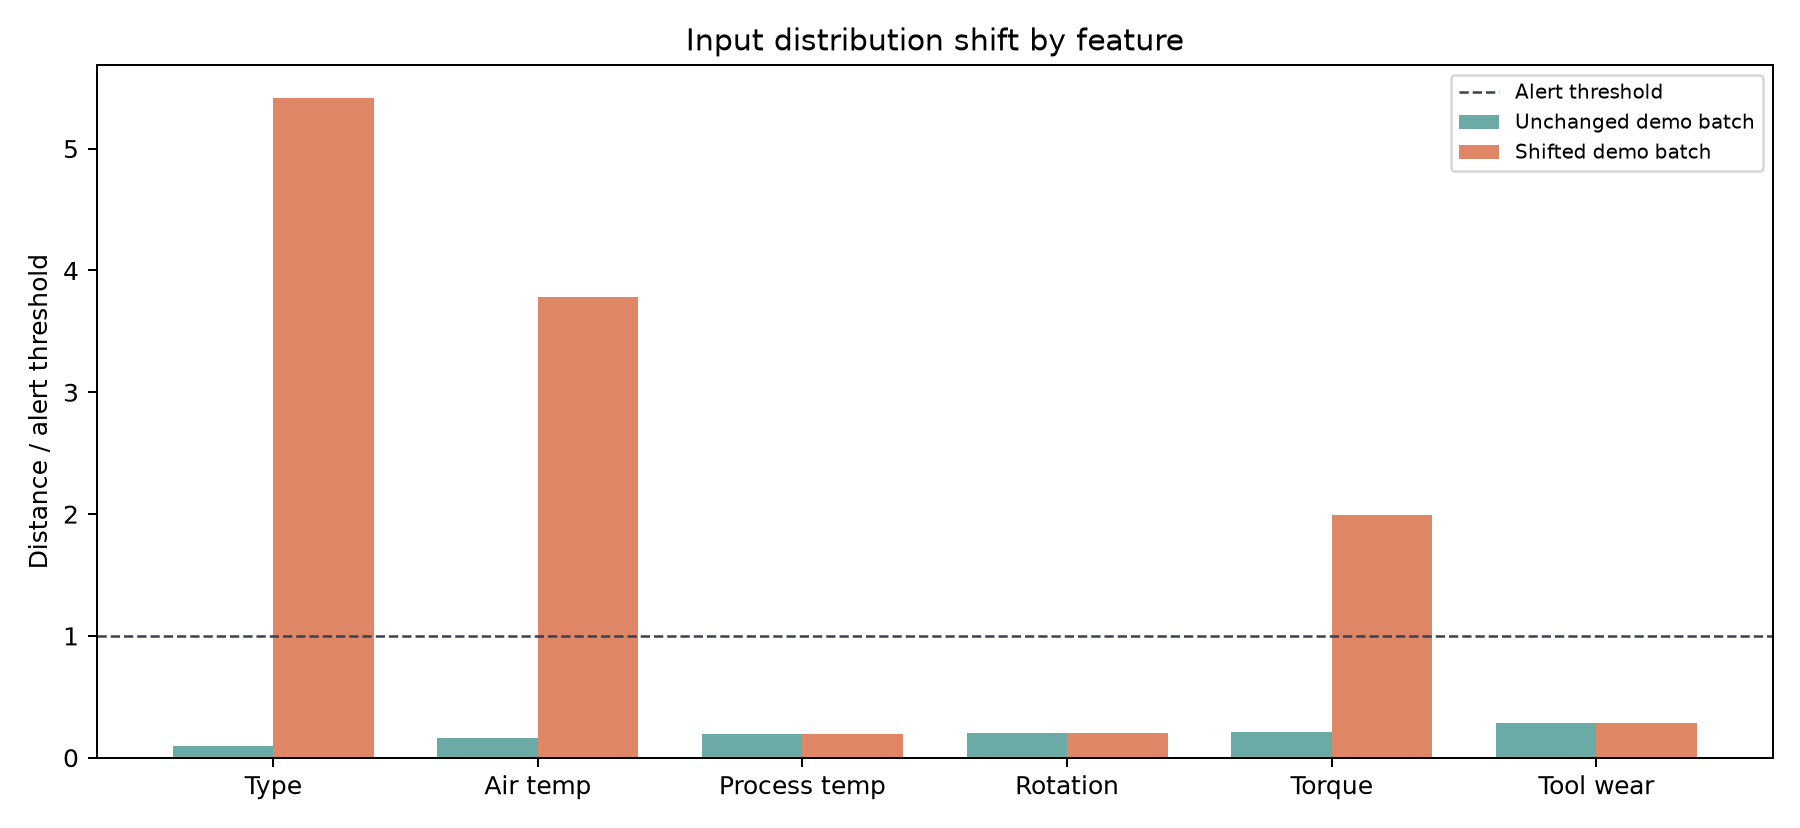
\includegraphics[width=.98\textwidth]{drift_scores.png}\caption{Thống kê so sánh từng thuộc tính giữa lô bình thường, lô dịch chuyển và tập train.}\label{fig:drift}\end{figure}

Một hệ thống phát hiện đúng ba biến được sửa là kiểm tra logic hữu ích. Nó không chứng minh ngưỡng hiện tại có tỷ lệ báo giả phù hợp trong dữ liệu thật. Lô bình thường là mẫu từ cùng nguồn, nên tương đối dễ đạt \src{ok}. Ngoài ra, monitor chỉ đo phân phối từng thuộc tính riêng lẻ; quan hệ giữa hai cảm biến có thể thay đổi mà các phân phối biên vẫn gần như cũ. Khi triển khai thật, cần theo dõi thêm tỷ lệ giá trị thiếu, miền hợp lệ theo thiết bị, tần suất dự đoán, nhãn đến trễ và chỉ số mô hình sau khi có nhãn.

\section{Kiểm tra khả năng tái tạo và vận hành}
Quy trình \src{dvc repro} làm rõ rằng dữ liệu, mã và cấu hình nào dẫn tới hiện vật. \src{dvc.lock} ghi trạng thái các giai đoạn; \src{metrics.json} ghi kết quả số; MLflow ghi lịch sử run; nguồn LaTeX trỏ vào những hiện vật này khi dựng bảng và hình. Khi API chạy, \src{/health} kiểm tra mô hình nạp được, còn \src{/predict} thực hiện một suy luận theo schema. Các thành phần này đã được thiết kế để kiểm tra những rủi ro khác nhau: DVC về phụ thuộc pipeline, MLflow về dấu vết thử nghiệm, API về hợp đồng phục vụ, monitor về dữ liệu đầu vào.

Tính tái tạo ở đây vẫn có điều kiện. Bước download cần UCI còn truy cập được; một số gói trong \src{pyproject.toml} có khoảng phiên bản; phần cứng và hệ điều hành khác có thể tạo sai khác số thực nhỏ. Tệp dữ liệu gốc có hash cụ thể nên sai khác nội dung sẽ được phát hiện. Với yêu cầu lặp lại chặt chẽ hơn, nhóm sẽ cố định lockfile môi trường, lưu dữ liệu và mô hình trong remote có phiên bản, đồng thời ghi commit Git vào mỗi MLflow run.

\section{Những gì kết quả chưa chứng minh}
AP và recall trên test phản ánh một phép chia ngẫu nhiên của dữ liệu tổng hợp. Chúng chưa đo khả năng khái quát sang nhà máy khác, dòng máy khác hoặc năm vận hành khác. Nhãn tại một bản ghi hiện tại cũng không cung cấp chân trời dự báo, vì vậy chưa thể tính ``phát hiện trước bao lâu''. Với một ứng dụng bảo trì thật, việc cảnh báo sau khi máy đã hỏng có thể không đáp ứng nhu cầu. Cần thu thập chuỗi thời gian trước sự cố, xác định mốc cảnh báo, loại bỏ mọi thông tin chỉ xuất hiện sau sự cố và kiểm tra theo thiết bị/thời gian.

Thử nghiệm drift chỉ minh họa phát hiện biến đổi đầu vào được cố ý chèn. Nó không xác nhận hiệu năng mô hình giảm khi có drift; có loại drift không ảnh hưởng đến nhãn, và cũng có sự thay đổi quan hệ $P(Y\mid X)$ mà các phân phối biên đầu vào không báo rõ. Không nên tự động huấn luyện lại chỉ vì một thống kê vượt ngưỡng. Hệ thống vận hành cần quy trình xem xét cảnh báo, lấy mẫu nhãn, so sánh mô hình mới với mô hình đang dùng và khả năng quay lại phiên bản trước.


\chapter{Kết luận và hướng phát triển}
\section{Kết quả đạt được}
Nhóm đã xây dựng một dự án MLOps từ dữ liệu \dataset{} đến dịch vụ dự đoán và báo cáo giám sát. Dữ liệu được tải và xác thực, sáu thuộc tính đầu vào được định nghĩa nhất quán, phép chia train/validation/test có phân tầng, ba ứng viên được so sánh theo AP, ngưỡng được chọn trên validation bằng $F_2$. XGBoost được chọn với ngưỡng 0,15; trên test, mô hình đạt AP 0,825 và phát hiện 54 trong 68 bản ghi hỏng. Bên cạnh mô hình, dự án có DVC, MLflow, FastAPI, Docker, GitHub Actions và chương trình tạo bằng chứng cho báo cáo.

Thử nghiệm monitor cho thấy lô bình thường trả \src{ok} và lô dịch chuyển trả \src{alert} ở đúng ba thuộc tính được sửa. Kết quả này xác nhận đường xử lý của bản mẫu ở tình huống kiểm tra đã thiết kế. Báo cáo trình bày đầy đủ nguồn gốc số liệu, ma trận nhầm lẫn và điều kiện của các ngưỡng, để người đọc có thể phân biệt số đo thực nghiệm với định hướng phát triển.

\section{Hạn chế}
Dữ liệu gốc là tổng hợp, không có thời gian hay lịch sử thiết bị, và nhãn mô tả trạng thái hỏng tại một quan sát. Do đó không thể dùng kết quả này để khẳng định khả năng cảnh báo sớm cho máy công nghiệp. Chỉ một phép chia dữ liệu và một bộ cấu hình cho mỗi thuật toán được thử; chưa có kiểm tra độ ổn định qua nhiều seed, kiểm định theo nhà máy hoặc đánh giá chi phí thực. Các ngưỡng giám sát là minh họa, chưa được hiệu chuẩn theo tần suất cảnh báo chấp nhận được.

Hạ tầng hiện tại phục vụ một máy cá nhân: DVC chưa có remote, MLflow dùng SQLite cục bộ, chưa có triển khai API công khai, lịch thu thập nhãn hay cơ chế huấn luyện lại tự động. CI kiểm tra mã nhưng không thay thế kiểm thử dữ liệu và mô hình ở môi trường triển khai. Những giới hạn này phù hợp với phạm vi bản mẫu học phần và là cơ sở xác định công việc tiếp theo.

\section{Hướng phát triển ưu tiên}
Ưu tiên đầu tiên là dữ liệu: thu thập chuỗi cảm biến theo thiết bị, thời điểm sự cố và khoảng thời gian cần báo trước. Cần thiết kế lại nhãn theo chân trời dự báo, chia tập theo thời gian hoặc thiết bị và đánh giá trên giai đoạn triển khai về sau. Sau đó, nhóm có thể so sánh thêm cách hiệu chuẩn xác suất, các ngưỡng theo chi phí thực và phép đo độ không chắc chắn của hiệu năng. Một đường chuẩn đơn giản và đáng tin nên tiếp tục được giữ khi tăng độ phức tạp mô hình.

Ưu tiên vận hành là lưu dữ liệu và mô hình vào remote có phiên bản, ghi commit và dấu băm vào MLflow, dựng tracking server dùng chung, kiểm tra image cùng hiện vật trước khi phát hành. Monitor cần kết nối với nhãn đến trễ và một quy trình phản hồi của người vận hành; cảnh báo drift nên dẫn tới điều tra thay vì tự động thay mô hình. Các bước này biến bản mẫu có thể chạy lại thành một hệ thống có kiểm soát thay đổi và có bằng chứng chất lượng sau triển khai.


\begin{thebibliography}{99}
\bibitem{uci2020} S. Matzka, ``AI4I 2020 Predictive Maintenance Dataset,'' UCI Machine Learning Repository, 2020. DOI: \href{https://doi.org/10.24432/C5HS5C}{10.24432/C5HS5C}. Truy cập ngày 25/11/2026.
\bibitem{matzka2020} S. Matzka, ``Explainable Artificial Intelligence for Predictive Maintenance Applications,'' \emph{2020 Third International Conference on Artificial Intelligence for Industries}, 2020. DOI: \href{https://doi.org/10.1109/AI4I49448.2020.00023}{10.1109/AI4I49448.2020.00023}.
\bibitem{saito2015} T. Saito và M. Rehmsmeier, ``The Precision-Recall Plot Is More Informative than the ROC Plot When Evaluating Binary Classifiers on Imbalanced Datasets,'' \emph{PLOS ONE}, 10(3), 2015. DOI: \href{https://doi.org/10.1371/journal.pone.0118432}{10.1371/journal.pone.0118432}.
\bibitem{sculley2015} D. Sculley và cộng sự, ``Hidden Technical Debt in Machine Learning Systems,'' \emph{Advances in Neural Information Processing Systems 28}, 2015. \url{https://proceedings.neurips.cc/paper/2015/hash/86df7dcfd896fcaf2674f757a2463eba-Abstract.html}.
\bibitem{breiman2001} L. Breiman, ``Random Forests,'' \emph{Machine Learning}, 45, 5--32, 2001. DOI: \href{https://doi.org/10.1023/A:1010933404324}{10.1023/A:1010933404324}.
\bibitem{chen2016} T. Chen và C. Guestrin, ``XGBoost: A Scalable Tree Boosting System,'' \emph{Proceedings of the 22nd ACM SIGKDD International Conference on Knowledge Discovery and Data Mining}, 2016. DOI: \href{https://doi.org/10.1145/2939672.2939785}{10.1145/2939672.2939785}.
\bibitem{dvc} DVC, ``Defining and Running Pipelines,'' tài liệu chính thức. \url{https://doc.dvc.org/user-guide/pipelines/running-pipelines}. Truy cập ngày 25/11/2026.
\bibitem{mlflow} MLflow, ``MLflow Tracking,'' tài liệu chính thức. \url{https://mlflow.org/docs/latest/tracking/}. Truy cập ngày 25/11/2026.
\bibitem{fastapi} FastAPI, ``First Steps,'' tài liệu chính thức. \url{https://fastapi.tiangolo.com/tutorial/first-steps/}. Truy cập ngày 25/11/2026.
\bibitem{docker} Docker, ``Dockerfile overview,'' tài liệu chính thức. \url{https://docs.docker.com/build/concepts/dockerfile/}. Truy cập ngày 25/11/2026.
\bibitem{actions} GitHub, ``GitHub Actions quickstart,'' tài liệu chính thức. \url{https://docs.github.com/en/actions/get-started/quickstart}. Truy cập ngày 25/11/2026.
\bibitem{scipyks} SciPy, ``scipy.stats.ks\_2samp,'' tài liệu API chính thức. \url{https://docs.scipy.org/doc/scipy/reference/generated/scipy.stats.ks_2samp.html}. Truy cập ngày 25/11/2026.
\bibitem{breck2017} E. Breck và cộng sự, ``The ML Test Score: A Rubric for ML Production Readiness and Technical Debt Reduction,'' Google Research, 2017. \url{https://research.google/pubs/the-ml-test-score-a-rubric-for-ml-production-readiness-and-technical-debt-reduction/}.
\end{thebibliography}


\appendix
\chapter{Hướng dẫn tái tạo thực nghiệm}
\section{Điều kiện chạy}
Máy cần Python từ 3.11 đến dưới 3.14, Git và kết nối đến nguồn UCI khi tải dữ liệu. Docker Desktop chỉ cần cho bước chạy API trong container. Các lệnh sau được viết theo PowerShell ở thư mục gốc repository. Việc cài package dùng \src{pyproject.toml}; môi trường chạy báo cáo cụ thể dùng Python 3.13.12. Nếu người đọc dùng phiên bản thư viện khác, cần so sánh kết quả trong \src{artifacts/metrics.json} thay vì giả định mọi chữ số thập phân giống nhau.

\begin{lstlisting}[language={},caption={Tạo môi trường và cài phụ thuộc}]
python -m venv .venv
.\.venv\Scripts\Activate.ps1
python -m pip install -e ".[train,report,dev]"
\end{lstlisting}
Sau cài đặt, có thể chạy \src{python -m pytest} để kiểm tra mã trước khi tạo hiện vật. Nếu PowerShell chặn kích hoạt script theo chính sách máy, có thể gọi trực tiếp tệp \src{python.exe} trong thư mục \src{.venv/Scripts} thay vì thay đổi chính sách toàn hệ thống.

\section{Tải dữ liệu và huấn luyện}
\begin{lstlisting}[language={},caption={Chạy pipeline và kiểm tra hiện vật}]
dvc repro
python -m predictive_maintenance.report
Get-Content artifacts/metrics.json
\end{lstlisting}
Lệnh \src{dvc repro} chạy hai stage theo phụ thuộc. Bước tải dữ liệu lấy CSV gốc và kiểm tra SHA-256. Bước train sinh ba tệp trong \src{artifacts}. Nếu đã có hiện vật và phụ thuộc không đổi, DVC có thể bỏ qua stage; muốn tái chạy để kiểm tra từ đầu cần dùng lựa chọn phù hợp của DVC và lưu ý rằng nguồn tải phải khả dụng. Khi chạy báo cáo bằng chứng, các lô giám sát ở phần kế tiếp cần được tạo trước nếu muốn kết quả giám sát đầy đủ.

\section{Tạo lô giám sát và kiểm tra cảnh báo}
\begin{lstlisting}[language={},caption={Tạo và so sánh hai lô demo}]
python -m predictive_maintenance.simulate \
  --output data/monitoring/normal.csv
python -m predictive_maintenance.monitor \
  --current data/monitoring/normal.csv \
  --output artifacts/monitoring/normal.json
python -m predictive_maintenance.simulate --drift \
  --output data/monitoring/drifted.csv
python -m predictive_maintenance.monitor \
  --current data/monitoring/drifted.csv \
  --output artifacts/monitoring/drifted.json
python -m predictive_maintenance.report
\end{lstlisting}
Các dấu nối dòng trong Listing trên minh họa cách trình bày; trong PowerShell nên chạy mỗi lệnh trên một dòng hoặc dùng ký tự nối dòng PowerShell. Cần đối chiếu \src{status} trong hai tệp JSON: bình thường là \src{ok}, dịch chuyển là \src{alert}. Tệp \src{reports/evidence.md} được tạo lại sau khi đủ hai báo cáo giám sát.

\section{Khởi chạy API}
\begin{lstlisting}[language={},caption={Chạy API trên máy và gọi thử}]
uvicorn predictive_maintenance.api:app \
  --host 127.0.0.1 --port 8000
\end{lstlisting}
Trong PowerShell khác, có thể gọi \src{Invoke-RestMethod} như README. \src{GET http://127.0.0.1:8000/health} trả \src{status: ok} nếu mô hình nạp được. Gửi yêu cầu thiếu \src{torque} hoặc \src{type} ngoài L/M/H sẽ bị xác thực từ chối. Điều này kiểm tra cấu trúc đầu vào, không phải bài kiểm tra độ chính xác mô hình. Tài liệu tương tác của FastAPI ở đường \src{/docs} khi server đang chạy.

\section{Biên dịch bản báo cáo}
\begin{lstlisting}[language={},caption={Tạo bảng, hình và biên dịch LaTeX}]
python latex-report/generate_assets.py
cd latex-report
latexmk -xelatex -interaction=nonstopmode \
  -halt-on-error -file-line-error \
  -outdir=build main.tex
\end{lstlisting}
Nguồn LaTeX dùng XeLaTeX để hiển thị tiếng Việt với Times New Roman. Script tạo hình kiểm tra dấu băm của CSV và tính nhất quán của hiện vật trước khi ghi các bảng trong \src{generated}. Nếu có thay đổi số liệu, cần chạy lại script trước bước biên dịch. PDF bàn giao nằm ở \src{output/pdf} trong repository; thư mục \src{build} chứa tệp trung gian.

\chapter{Hợp đồng dữ liệu và API}
\section{Schema đầu vào dự đoán}
\begin{longtable}{p{4.2cm}p{3cm}p{6.5cm}}
\caption{Các trường JSON của \src{POST /predict}}\label{tab:api-schema}\\
\toprule Trường & Kiểu / điều kiện & Ánh xạ đến cột huấn luyện\\\midrule\endfirsthead
\toprule Trường & Kiểu / điều kiện & Ánh xạ đến cột huấn luyện\\\midrule\endhead
\src{type} & L, M hoặc H & \src{Type}\\
\src{air_temperature} & số thực $>0$ & \src{Air temperature [K]}\\
\src{process_temperature} & số thực $>0$ & \src{Process temperature [K]}\\
\src{rotational_speed} & số nguyên $>0$ & \src{Rotational speed [rpm]}\\
\src{torque} & số thực $\geq0$ & \src{Torque [Nm]}\\
\src{tool_wear} & số nguyên $\geq0$ & \src{Tool wear [min]}\\\bottomrule
\end{longtable}
API trả một xác suất thực trong đoạn $[0,1]$, một giá trị Boolean về cảnh báo và ngưỡng đọc từ bundle. Không có trường định danh thiết bị hoặc thời điểm, do đó API không lưu chuỗi lịch sử. Muốn dùng trong một hệ thống thực, cần định nghĩa phiên bản schema, đơn vị đo và phạm vi hợp lý theo từng dòng máy, đồng thời gắn định danh yêu cầu để đối chiếu khi có nhãn đến trễ.

\section{Schema lô giám sát}
CSV giám sát phải có đủ sáu cột tên như Bảng~\ref{tab:features}. Monitor không cần cột nhãn. Nó chấp nhận cột bổ sung nhưng chỉ chọn sáu trường đã định. Tham chiếu đọc từ \src{artifacts/reference.csv}; dữ liệu mới đọc qua \src{--current}. Tệp tham chiếu phải có \src{Type} hợp lệ và mọi giá trị số hữu hạn. Với lô mới, giá trị không hợp lệ được đếm vào \src{quality_issues}; nếu một cột hoàn toàn không có giá trị số hợp lệ thì thống kê drift của cột đó là \src{null}. Lô dưới 100 dòng bị đánh dấu vấn đề chất lượng. Trạng thái \src{alert} cũng được bật khi có lỗi chất lượng dù không phát hiện drift.

\section{Giải thích các trường trong báo cáo giám sát}
Tệp JSON có \src{reference_rows}, \src{current_rows}, \src{drift_detected}, \src{drifted_features}, \src{data_quality_alert}, \src{quality_issues}, \src{status} và bản ghi \src{features} cho từng thuộc tính. Với Type, bản ghi chứa khoảng cách TV, ngưỡng và số hàng không hợp lệ. Với biến số, nó chứa thống kê KS, p-value, ngưỡng, trung bình tham chiếu, trung bình lô mới và số hàng không hợp lệ. Cấu trúc này cho phép phân biệt thay đổi phân phối với trục trặc trong dữ liệu nhập.

\chapter{Đối chiếu số liệu và giới hạn diễn giải}
\section{Các phép kiểm tra số học}
Các tỷ lệ trong báo cáo có thể kiểm tra từ số đếm gốc. Tỷ lệ hỏng toàn bộ là $339/10000=0,0339$. Tỷ lệ theo các tập lần lượt là $217/6400\approx0,0339$, $54/1600=0,03375$ và $68/2000=0,034$. Ma trận test có tổng $1898+34+14+54=2000$. Số dương thực là $14+54=68$, số âm thực là $1898+34=1932$. Số cảnh báo là $34+54=88$. Precision và recall tính từ các số đếm này khớp với metric lưu.

\section{Ý nghĩa của average precision}
Trong scikit-learn, average precision là tổng có trọng số của precision tại các mức thay đổi recall. Nó không bằng precision ở ngưỡng 0,15. Khi báo cáo so sánh AP giữa ba mô hình, nhóm chỉ kết luận về khả năng sắp xếp bản ghi trong phép chia đang dùng. Nếu người vận hành chỉ có năng lực kiểm tra một số ít máy mỗi ngày, cần thêm chỉ số như precision ở top-$k$, tỷ lệ cảnh báo/ngày và chi phí theo lịch sản xuất. Những thông tin này chưa có trong dữ liệu hiện tại.

\section{Các nguồn sai lệch cần chú ý}
Nguồn sai lệch thứ nhất là dữ liệu tổng hợp: cấu trúc quan hệ có thể đơn giản hơn thực tế. Nguồn thứ hai là chia ngẫu nhiên trên bản ghi thay vì chia theo máy hoặc thời gian; kết quả không đại diện cho máy mới hay tương lai. Nguồn thứ ba là lựa chọn cấu hình mô hình hạn chế; điểm XGBoost là điểm của một cấu hình cụ thể. Nguồn thứ tư là tối ưu ngưỡng theo một validation có 54 trường hợp hỏng; ngưỡng có thể dao động khi đổi mẫu. Nguồn thứ năm là monitor được thử với dịch chuyển lớn, có chủ đích; nó chưa được đo tỷ lệ báo giả qua nhiều lô bình thường.

\section{Tiêu chí chuyển sang thử nghiệm thực tế}
Trước khi thử trên thiết bị thật, cần xác định câu hỏi vận hành: cảnh báo trước bao nhiêu giờ hoặc chu kỳ, ai nhận cảnh báo, hành động kiểm tra nào được thực hiện và chi phí của mỗi hành động. Sau đó cần thu thập dữ liệu có dấu thời gian, dữ liệu sự cố đã xác nhận và thông tin thiết bị. Mô hình phải được đánh giá trên giai đoạn sau thời điểm huấn luyện, tốt hơn nữa trên thiết bị không xuất hiện trong train. Trong thử nghiệm bóng, hệ thống có thể ghi dự đoán mà chưa chi phối hành động, để đo tỷ lệ cảnh báo và chất lượng khi nhãn đến. Chỉ sau các bước này mới có cơ sở quyết định triển khai có tác động đến sản xuất.

\chapter{Quy trình kiểm tra một cảnh báo vận hành}
\section{Khi API không nạp được mô hình}
Nếu \src{/health} trả 503, trước tiên kiểm tra tệp \src{artifacts/model.joblib} có tồn tại tại đường dẫn được cấu hình bởi \src{MODEL_PATH} hay không. Trong container, kiểm tra volume \src{artifacts} đã được gắn đúng vào \src{/app/artifacts} ở chế độ đọc. Tiếp theo kiểm tra phiên bản các thư viện dùng để tạo và nạp bundle; một hiện vật joblib tạo ở môi trường khác có thể không tương thích. Chỉ khi mô hình nạp được mới thực hiện thử \src{/predict} bằng một bản ghi có giá trị hợp lệ. Không nên thay thế lỗi 503 bằng một xác suất mặc định, vì như vậy người nhận API không biết dự đoán đã không được tính.

Sau khi sửa vấn đề nạp mô hình, cần ghi phiên bản mã, hash hiện vật và thời điểm khởi động lại. Bản mẫu hiện chỉ thực hiện kiểm tra nạp tệp; một quy trình vận hành thật nên có bài kiểm tra dự đoán chuẩn với đầu vào và đầu ra kỳ vọng trong sai số cho phép. Kiểm tra này giúp phát hiện trường hợp mô hình nạp được nhưng schema hoặc phiên bản tiền xử lý không trùng với môi trường huấn luyện.

\section{Khi monitor trả trạng thái alert}
Trước tiên đọc \src{data_quality_alert} và \src{quality_issues}. Nếu có giá trị thiếu, không hữu hạn, \src{Type} lạ hoặc lô dưới 100 dòng, cần kiểm tra nguồn dữ liệu trước khi diễn giải thống kê drift. Các thống kê được tính sau khi loại giá trị số không hợp lệ; một lô có nhiều giá trị lỗi có thể cho kết quả phân phối không đại diện. Sau đó đọc \src{drifted_features} và chi tiết từng thuộc tính để xác định thay đổi nằm ở tần suất danh mục hay phân phối biến số.

Với cảnh báo Type, so sánh tỷ lệ L/M/H của lô mới và tập train để xem nguồn sản phẩm có thay đổi thật hay do lỗi ánh xạ mã. Với cảnh báo nhiệt độ hoặc mô-men, kiểm tra đơn vị đo, cấu hình cảm biến và điều kiện vận hành trước khi kết luận máy có vấn đề. Ví dụ, cộng nhầm độ C vào dữ liệu đã ghi bằng K sẽ tạo thay đổi lớn mà không phản ánh hiện tượng vật lý mới. Nếu dữ liệu hợp lệ, có thể tăng tần suất lấy mẫu nhãn và kiểm tra đầu ra mô hình trên các ca được chuyên gia xác nhận.

\section{Quyết định sau khi xác minh cảnh báo}
Một cảnh báo đầu vào không đủ để đổi mô hình. Nếu chỉ thay đổi cơ cấu sản phẩm nhưng chất lượng dự đoán vẫn đạt yêu cầu, có thể tiếp tục theo dõi. Nếu precision hoặc recall đo từ nhãn thật giảm, cần kiểm tra xem lỗi đến từ dữ liệu thu thập, thay đổi quy trình hay quan hệ giữa cảm biến và sự cố. Khi có mô hình ứng viên mới, đánh giá nó trên một tập thời gian gần đây không dùng để huấn luyện, so sánh chi phí cảnh báo và thử nghiệm bóng. Việc phát hành phải lưu được phiên bản cũ và có cách quay lại nếu tỷ lệ lỗi tăng.

Bản mẫu chưa tự động hóa các quyết định này. Tệp JSON của monitor là một tín hiệu đầu vào cho người phụ trách, không phải mệnh lệnh huấn luyện lại. Quy trình thủ công có ghi nhận bằng chứng là lựa chọn phù hợp khi dữ liệu nhãn và mục tiêu vận hành chưa đủ rõ để đặt các ngưỡng tự động đáng tin.


\end{document}
